\chapter{Modelagem do Sistema}
\label{cap:modelagem}

Este capítulo apresenta a modelagem e a arquitetura do sistema IGRIS, descrevendo as decisões de projeto que conectam os requisitos identificados à implementação técnica. A modelagem é organizada em quatro perspectivas complementares: a arquitetura do sistema e seus componentes; a modelagem funcional e comportamental, representada pelos atores e casos de uso; a modelagem estrutural, expressa pelo diagrama de classes; e a modelagem de dados, formalizada pelo Modelo Entidade-Relacionamento e pelo dicionário de dados.

\section{Arquitetura do Sistema}
\label{sec:4.1}

O IGRIS adota um Monolito Modular com Adaptadores de Microsserviços, combinando a organização interna por módulos de domínio com o desacoplamento externo de componentes computacionalmente intensivos. O núcleo da aplicação é um único processo Spring Boot organizado em módulos coesos acadêmico, usuário, instituição, grade, segurança e comum, que se comunicam internamente sem latência de rede. Para a execução do Algoritmo Genético, o sistema delega o processamento a microsserviços independentes via adaptadores HTTP, isolando a lógica pesada de otimização sem comprometer a responsividade da API principal \cite[p.~15--16]{newman2021}.

A comunicação entre o Backend Core e os microsserviços ocorre de forma síncrona: o backend monta um \textit{payload} JSON com disponibilidades, matrizes, turmas e parâmetros do algoritmo, envia por HTTP POST ao microsserviço selecionado e recebe uma resposta estruturada contendo a grade otimizada, métricas de execução e lista de conflitos. Os parâmetros do algoritmo são armazenados na tabela \texttt{config\_sistema} e carregados em cache, permitindo ajuste em tempo de execução sem reinicialização \cite[p.~3]{newman2021}.

A arquitetura é composta por quatro serviços principais:

\begin{itemize}
  \item \textbf{Igris (Backend Core):} API principal em Java 17 com Spring Boot 3.5. Gerencia todas as operações CRUD do domínio acadêmico, autenticação JWT, controle de acesso RBAC e orquestra as chamadas aos microsserviços de otimização. É o único componente com acesso direto ao banco de dados PostgreSQL 15.
  \item \textbf{Sunny:} Microsserviço de geração de grade em Java com Spring Boot, implementando o Algoritmo Genético no paradigma orientado a objetos.
  \item \textbf{Morpheus:} Microsserviço equivalente em Python com Flask, implementando o mesmo algoritmo no paradigma funcional, com parada antecipada e melhoria local explícita.
  \item \textbf{Rocket:} Microsserviço em Go, implementando o AG com modelo de concorrência baseado em \textit{goroutines} e \textit{channels} (CSP). Representa o paradigma concorrente no benchmark comparativo \cite{coxbuday2017}.
\end{itemize}

Todos os componentes são containerizados via Docker e se comunicam pela rede interna \texttt{igris-network}, sem exposição direta ao exterior. O frontend React acessa exclusivamente o Backend Core na porta 8080 \cite[p.~20]{newman2021}.

\begin{figure}[H]
\centering
\caption{Arquitetura do sistema IGRIS}
\label{fig:arquitetura}

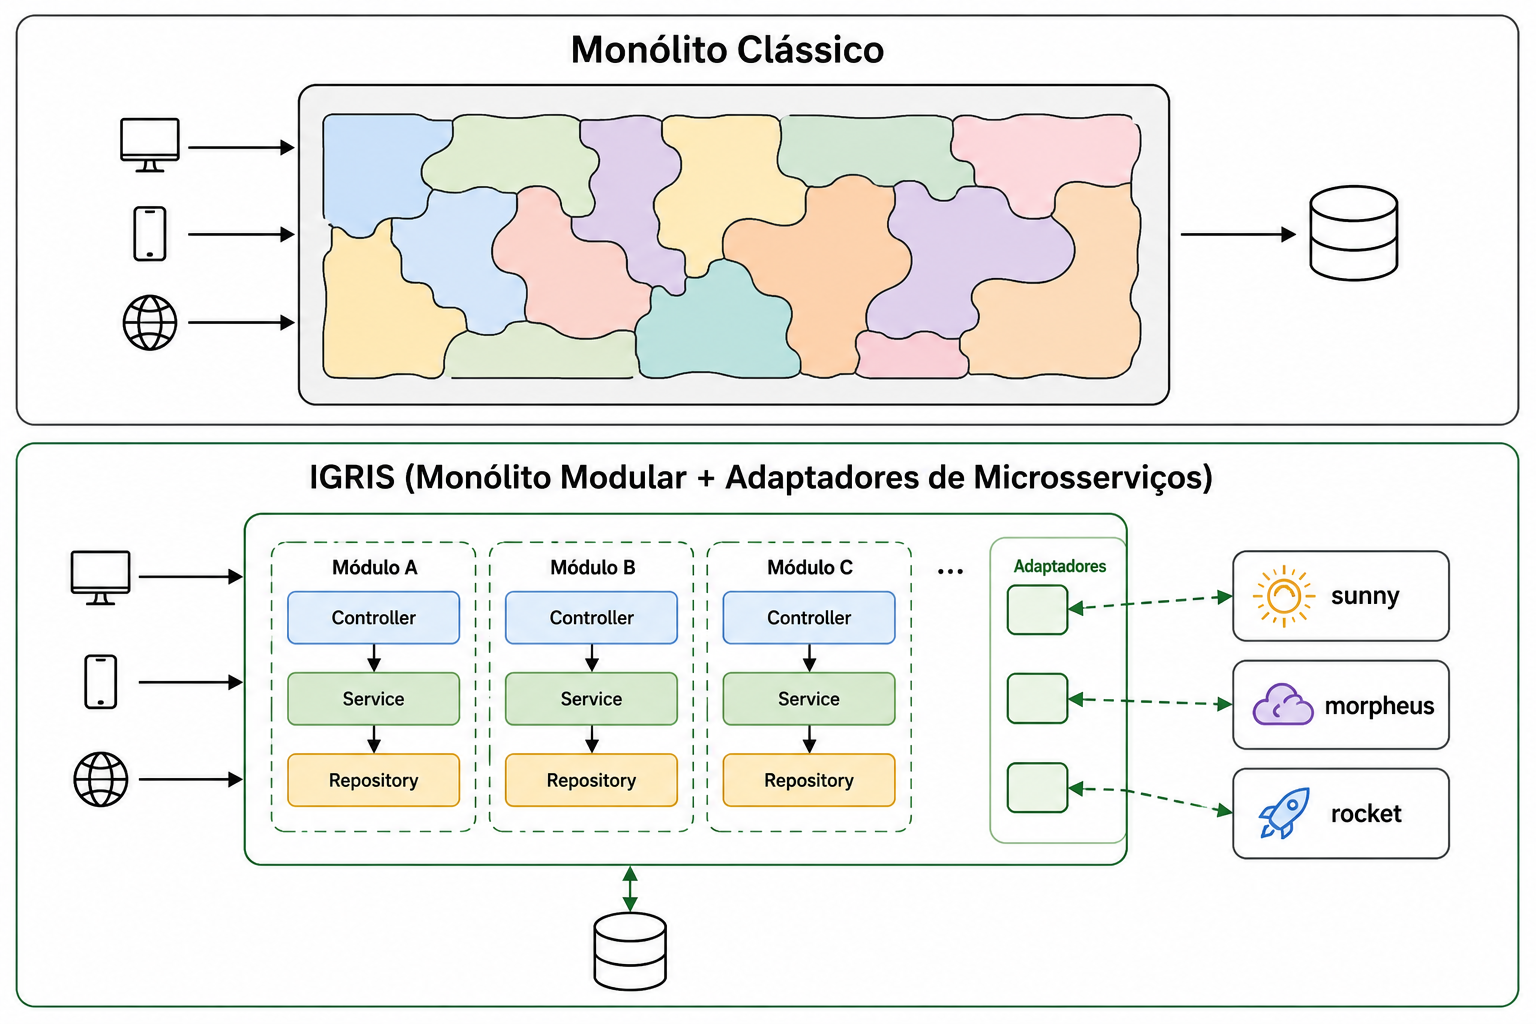
\includegraphics[width=0.85\textwidth]{figuras/Figura_8_ilustracaoArquitetura.png}

\vspace{0.2cm}
\fonteautores
\end{figure}
\section{Modelagem Funcional e Comportamental}
\label{sec:4.2}

A modelagem funcional tem como objetivo descrever as interações entre os usuários e o sistema, delimitando o escopo das funcionalidades e o comportamento esperado frente a diferentes cenários de uso. Segundo \citeonline{pressman2016}, essa etapa é fundamental para validar se os requisitos levantados correspondem às expectativas dos stakeholders, servindo como guia visual e textual para o desenvolvimento.

\subsection{Atores do Sistema}
\label{subsec:4.2.1}

O sistema IGRIS é composto por cinco atores, cada um com responsabilidades bem delimitadas conforme ilustrado no Diagrama de Casos de Uso.

O usuário representa o ator base do sistema. Todo acesso ao IGRIS é autenticado, cabendo ao usuário as operações comuns: autenticar-se, selecionar ou trocar de perfil, recuperar senha, realizar cadastro via link de convite e enviar feedback.

O coordenador é o ator gestor do fluxo acadêmico. Suas responsabilidades abrangem manter a disponibilidade dos professores, gerenciar disciplinas, turmas, cursos e matrizes, vincular disciplinas a cursos, manter turnos e dias letivos, gerar o link de cadastro de professores, além de gerar, salvar e visualizar a grade horária.

O professor alimenta o sistema com suas próprias informações: mantém sua disponibilidade de horários, registra as disciplinas que leciona e visualiza a própria grade gerada.

A instituição é responsável por operações de gestão de coordenadores: manter coordenadores e coordenações vinculadas à instituição.

O administrador do sistema possui acesso privilegiado: concede ou revoga perfis de acesso, mantém configurações globais do sistema, gerencia instituições e usuários, visualiza feedbacks e mantém as configurações de geração de grade, incluindo os parâmetros matemáticos dos microsserviços.

\subsection{Diagrama de Casos de Uso}
\label{subsec:4.2.2}

O Diagrama de Casos de Uso do IGRIS representa graficamente todas as interações possíveis entre os cinco atores do sistema e suas respectivas funcionalidades, organizadas por perfil de acesso e nível de responsabilidade. O diagrama consolida em uma única visão as operações de cada ator: desde as funcionalidades comuns ao Usuário (autenticação, seleção de perfil, feedback), passando pelas responsabilidades do Coordenador (gestão acadêmica completa e geração de grade), do Professor (disponibilidade e disciplinas lecionadas), da Instituição (gestão de coordenação) e do Administrador do Sistema (configuração e controle de acesso).

\begin{figure}[p]
\centering
\caption{Diagrama de Casos de Uso do IGRIS}
\label{fig:casos_de_uso}
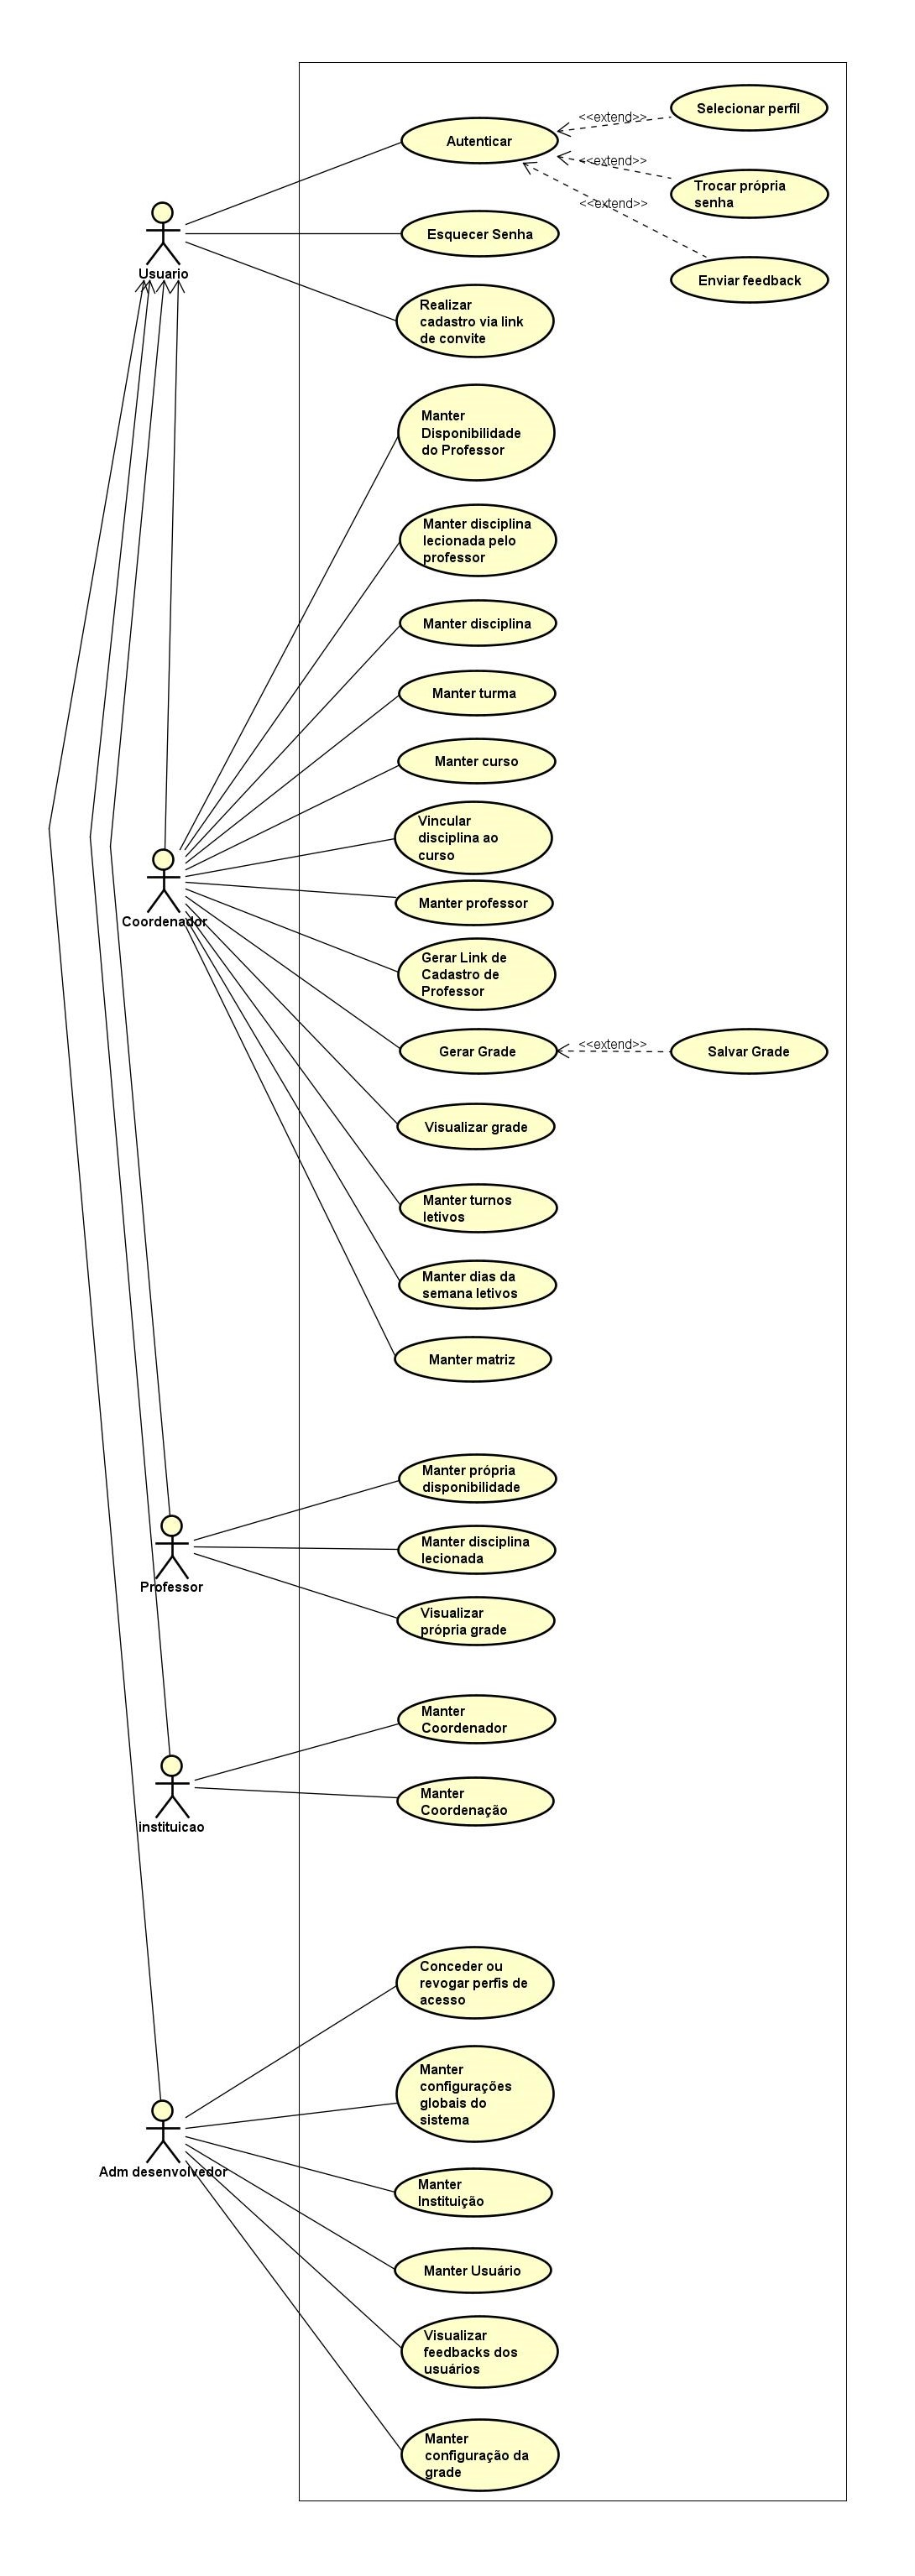
\includegraphics[width=\textwidth,height=0.86\textheight,keepaspectratio]{figuras/Figura_9_Diagrama de casos de uso.jpg}
\fonteautores
\end{figure}

\clearpage

\subsection{Descrição dos Casos de Uso}
\label{subsec:4.2.3}

Para eliminar ambiguidades inerentes à representação gráfica, os casos de uso foram detalhados textualmente seguindo o modelo de especificação padrão, com descrição, ator, pré-condição, pós-condição e fluxo principal de interação. Os Quadros de UC01 a UC33 apresentam a especificação completa de cada caso de uso do sistema.

% Tabela 3
\vspace{\baselineskip}

\Needspace{0.48\textheight}
\begin{longtable}{|L{4.5cm}|L{10.5cm}|}
\caption{Especificação do Caso de Uso: UC01 -- Autenticar} \\
\hline
\textbf{Nome do caso de uso} & \textbf{UC01 -- Autenticar} \\
\hline
\endfirsthead
\hline
\textbf{Nome do caso de uso} & \textbf{UC01 -- Autenticar} \\
\hline
\endhead
Descrição       & Permite que o usuário acesse o sistema de forma segura. \\
\hline
Ator            & Usuário \\
\hline
Pré-condição    & O usuário deve possuir um cadastro válido. \\
\hline
Pós-condição    & O usuário é logado no sistema e o token JWT é injetado. \\
\hline
Fluxo Principal & Ação do Ator: Informa login e senha e clica em entrar. Ação do Sistema: Valida credenciais no banco, gera o token de acesso e redireciona o usuário. \\
\hline
\end{longtable}

\fonteautores

% Tabela 4
\vspace{\baselineskip}

\Needspace{0.48\textheight}
\begin{longtable}{|L{4.5cm}|L{10.5cm}|}
\caption{Especificação do Caso de Uso: UC02 -- Selecionar/Trocar Perfil} \\
\hline
\textbf{Nome do caso de uso} & \textbf{UC02 -- Selecionar/Trocar Perfil} \\
\hline
\endfirsthead
\hline
\textbf{Nome do caso de uso} & \textbf{UC02 -- Selecionar/Trocar Perfil} \\
\hline
\endhead
Descrição       & Permite alterar o papel ativo na sessão (ex: trocar a visão de Professor para Coordenador). \\
\hline
Ator            & Usuário (Autenticado) \\
\hline
Pré-condição    & O usuário deve possuir múltiplos vínculos de perfis ativos. \\
\hline
Pós-condição    & O sistema reemite o token JWT com as permissões do novo perfil selecionado. \\
\hline
Fluxo Principal & Ação do Ator: Seleciona um novo perfil na interface e confirma. Ação do Sistema: Invalida o contexto anterior, emite novo token JWT e recarrega a página. \\
\hline
\end{longtable}

\fonteautores

% Tabela 5
\vspace{\baselineskip}

\Needspace{0.48\textheight}
\begin{longtable}{|L{4.5cm}|L{10.5cm}|}
\caption{Especificação do Caso de Uso: UC03 -- Trocar Própria Senha} \\
\hline
\textbf{Nome do caso de uso} & \textbf{UC03 -- Trocar Própria Senha} \\
\hline
\endfirsthead
\hline
\textbf{Nome do caso de uso} & \textbf{UC03 -- Trocar Própria Senha} \\
\hline
\endhead
Descrição       & Permite que o usuário altere sua senha por motivos de segurança. \\
\hline
Ator            & Usuário (Autenticado) \\
\hline
Pré-condição    & O usuário deve estar logado e saber sua senha atual. \\
\hline
Pós-condição    & A senha atual é substituída pela nova senha criptografada. \\
\hline
Fluxo Principal & Ação do Ator: Informa a senha atual e a nova senha desejada. Ação do Sistema: Valida a senha atual e criptografa e salva a nova. \\
\hline
\end{longtable}

\fonteautores

% Tabela 6
\vspace{\baselineskip}

\Needspace{0.48\textheight}
\begin{longtable}{|L{4.5cm}|L{10.5cm}|}
\caption{Especificação do Caso de Uso: UC04 -- Enviar Feedback} \\
\hline
\textbf{Nome do caso de uso} & \textbf{UC04 -- Enviar Feedback} \\
\hline
\endfirsthead
\hline
\textbf{Nome do caso de uso} & \textbf{UC04 -- Enviar Feedback} \\
\hline
\endhead
Descrição       & Enviar sugestões ou reportar bugs do sistema para os administradores. \\
\hline
Ator            & Usuário (Autenticado) \\
\hline
Pré-condição    & Estar logado no sistema. \\
\hline
Pós-condição    & O feedback é registrado na base atrelado ao usuário remetente. \\
\hline
Fluxo Principal & Ação do Ator: Seleciona a categoria, digita a mensagem e envia. Ação do Sistema: Salva o feedback no banco de dados. \\
\hline
\end{longtable}

\fonteautores

% Tabela 7
\vspace{\baselineskip}

\Needspace{0.48\textheight}
\begin{longtable}{|L{4.5cm}|L{10.5cm}|}
\caption{Especificação do Caso de Uso: UC05 -- Esquecer Senha} \\
\hline
\textbf{Nome do caso de uso} & \textbf{UC05 -- Esquecer Senha} \\
\hline
\endfirsthead
\hline
\textbf{Nome do caso de uso} & \textbf{UC05 -- Esquecer Senha} \\
\hline
\endhead
Descrição       & Permite ao usuário recuperar o acesso através de um link enviado por e-mail. \\
\hline
Ator            & Usuário \\
\hline
Pré-condição    & O usuário não consegue logar, mas possui acesso ao seu e-mail cadastrado. \\
\hline
Pós-condição    & Uma nova senha é cadastrada para o usuário. \\
\hline
Fluxo Principal & Ação do Ator: Solicita recuperação informando e-mail. Acessa o link e digita a nova senha. Ação do Sistema: Envia o e-mail com token. Valida o token e atualiza a senha no banco. \\
\hline
\end{longtable}

\fonteautores

% Tabela 8
\vspace{\baselineskip}

\Needspace{0.48\textheight}
\begin{longtable}{|L{4.5cm}|L{10.5cm}|}
\caption{Especificação do Caso de Uso: UC06 -- Realizar Cadastro via Link de Convite} \\
\hline
\textbf{Nome do caso de uso} & \textbf{UC06 -- Realizar Cadastro via Link de Convite} \\
\hline
\endfirsthead
\hline
\textbf{Nome do caso de uso} & \textbf{UC06 -- Realizar Cadastro via Link de Convite} \\
\hline
\endhead
Descrição       & Cadastro facilitado onde o professor já entra vinculado à faculdade. \\
\hline
Ator            & Usuário (Visitante/Professor) \\
\hline
Pré-condição    & Possuir um link/token de convite válido gerado por um coordenador. \\
\hline
Pós-condição    & Conta criada já com o perfil de Professor vinculado à instituição de origem do link. \\
\hline
Fluxo Principal & Ação do Ator: Acessa o link e preenche a senha e dados faltantes. Ação do Sistema: Valida o token do link, cria o usuário, atribui o perfil ACESSO\_PROFESSOR e expira o link. \\
\hline
\end{longtable}

\fonteautores

% Tabela 9
\vspace{\baselineskip}

\Needspace{0.48\textheight}
\begin{longtable}{|L{4.5cm}|L{10.5cm}|}
\caption{Especificação do Caso de Uso: UC07 -- Manter Disponibilidade do Professor} \\
\hline
\textbf{Nome do caso de uso} & \textbf{UC07 -- Manter Disponibilidade do Professor} \\
\hline
\endfirsthead
\hline
\textbf{Nome do caso de uso} & \textbf{UC07 -- Manter Disponibilidade do Professor} \\
\hline
\endhead
Descrição       & Permite ao coordenador visualizar e, se necessário, intervir na disponibilidade de tempo informada pelos professores. \\
\hline
Ator            & Coordenador \\
\hline
Pré-condição    & Professores devem possuir cadastro e vínculos na instituição. \\
\hline
Pós-condição    & A malha de disponibilidade dos professores fica pronta para o algoritmo. \\
\hline
Fluxo Principal & Ação do Ator: Consulta ou ajusta os dias/horários livres de um professor. Ação do Sistema: Salva a entidade Disponibilidade. \\
\hline
\end{longtable}

\fonteautores

% Tabela 10
\vspace{\baselineskip}

\Needspace{0.48\textheight}
\begin{longtable}{|L{4.5cm}|L{10.5cm}|}
\caption{Especificação do Caso de Uso: UC08 -- Manter Disciplina Lecionada pelo Professor} \\
\hline
\textbf{Nome do caso de uso} & \textbf{UC08 -- Manter Disciplina Lecionada pelo Professor} \\
\hline
\endfirsthead
\hline
\textbf{Nome do caso de uso} & \textbf{UC08 -- Manter Disciplina Lecionada pelo Professor} \\
\hline
\endhead
Descrição       & Permite ao coordenador gerenciar a equipe de professores e o que eles podem lecionar. \\
\hline
Ator            & Coordenador \\
\hline
Pré-condição    & Professores devem estar cadastrados na instituição. \\
\hline
Pós-condição    & Professor é mantido e vínculos com disciplinas são atualizados. \\
\hline
Fluxo Principal & Ação do Ator: Seleciona um professor e marca as disciplinas nas quais ele tem domínio. Ação do Sistema: Salva os registros na entidade UsuarioDisciplina. \\
\hline
\end{longtable}

\fonteautores

% Tabela 11
\vspace{\baselineskip}

\Needspace{0.48\textheight}
\begin{longtable}{|L{4.5cm}|L{10.5cm}|}
\caption{Especificação do Caso de Uso: UC09 -- Manter Disciplina} \\
\hline
\textbf{Nome do caso de uso} & \textbf{UC09 -- Manter Disciplina} \\
\hline
\endfirsthead
\hline
\textbf{Nome do caso de uso} & \textbf{UC09 -- Manter Disciplina} \\
\hline
\endhead
Descrição       & Permite gerenciar o catálogo global de disciplinas da coordenação. \\
\hline
Ator            & Coordenador \\
\hline
Pré-condição    & Estar logado como Coordenador. \\
\hline
Pós-condição    & A disciplina passa a existir no catálogo. \\
\hline
Fluxo Principal & Ação do Ator: Insere nome e carga horária da disciplina. Ação do Sistema: Persiste a disciplina no banco. \\
\hline
\end{longtable}

\fonteautores

% Tabela 12
\vspace{\baselineskip}

\Needspace{0.48\textheight}
\begin{longtable}{|L{4.5cm}|L{10.5cm}|}
\caption{Especificação do Caso de Uso: UC10 -- Manter Turma} \\
\hline
\textbf{Nome do caso de uso} & \textbf{UC10 -- Manter Turma} \\
\hline
\endfirsthead
\hline
\textbf{Nome do caso de uso} & \textbf{UC10 -- Manter Turma} \\
\hline
\endhead
Descrição       & Permite criar turmas de um curso para um determinado semestre/ano. \\
\hline
Ator            & Coordenador \\
\hline
Pré-condição    & Curso e Turno devem estar cadastrados. \\
\hline
Pós-condição    & Turma é instanciada e pronta para receber alunos/matrizes. \\
\hline
Fluxo Principal & Ação do Ator: Informa nome, curso, turno, semestre e ano. Ação do Sistema: Salva a entidade Turma vinculada à coordenação. \\
\hline
\end{longtable}

\fonteautores

% Tabela 13
\vspace{\baselineskip}

\Needspace{0.48\textheight}
\begin{longtable}{|L{4.5cm}|L{10.5cm}|}
\caption{Especificação do Caso de Uso: UC11 -- Manter Curso} \\
\hline
\textbf{Nome do caso de uso} & \textbf{UC11 -- Manter Curso} \\
\hline
\endfirsthead
\hline
\textbf{Nome do caso de uso} & \textbf{UC11 -- Manter Curso} \\
\hline
\endhead
Descrição       & Permite gerenciar os cursos oferecidos pela coordenação. \\
\hline
Ator            & Coordenador \\
\hline
Pré-condição    & Estar logado com o perfil de Coordenador. \\
\hline
Pós-condição    & Curso é criado, alterado ou removido logicamente. \\
\hline
Fluxo Principal & Ação do Ator: Preenche os dados do curso e solicita salvar. Ação do Sistema: Valida os dados e salva o curso atrelado à instituição/coordenação. \\
\hline
\end{longtable}

\fonteautores

% Tabela 14
\vspace{\baselineskip}

\Needspace{0.48\textheight}
\begin{longtable}{|L{4.5cm}|L{10.5cm}|}
\caption{Especificação do Caso de Uso: UC12 -- Vincular Disciplina ao Curso} \\
\hline
\textbf{Nome do caso de uso} & \textbf{UC12 -- Vincular Disciplina ao Curso} \\
\hline
\endfirsthead
\hline
\textbf{Nome do caso de uso} & \textbf{UC12 -- Vincular Disciplina ao Curso} \\
\hline
\endhead
Descrição       & Permite definir quais disciplinas fazem parte do catálogo de um curso. \\
\hline
Ator            & Coordenador \\
\hline
Pré-condição    & Curso e Disciplina devem existir. \\
\hline
Pós-condição    & Criado o relacionamento na tabela DisciplinaCurso. \\
\hline
Fluxo Principal & Ação do Ator: Seleciona o curso e marca as disciplinas pertencentes a ele. Ação do Sistema: Salva os vínculos na tabela de junção. \\
\hline
\end{longtable}

\fonteautores

% Tabela 15
\vspace{\baselineskip}

\Needspace{0.48\textheight}
\begin{longtable}{|L{4.5cm}|L{10.5cm}|}
\caption{Especificação do Caso de Uso: UC13 -- Manter Professor} \\
\hline
\textbf{Nome do caso de uso} & \textbf{UC13 -- Manter Professor} \\
\hline
\endfirsthead
\hline
\textbf{Nome do caso de uso} & \textbf{UC13 -- Manter Professor} \\
\hline
\endhead
Descrição       & Permite gerenciar os dados cadastrais básicos dos professores da instituição. \\
\hline
Ator            & Coordenador \\
\hline
Pré-condição    & Ter permissão de Coordenador. \\
\hline
Pós-condição    & Dados do professor são atualizados/cadastrados. \\
\hline
Fluxo Principal & Ação do Ator: Altera informações do professor. Ação do Sistema: Atualiza o cadastro no banco. \\
\hline
\end{longtable}

\fonteautores

% Tabela 16
\vspace{\baselineskip}

\Needspace{0.48\textheight}
\begin{longtable}{|L{4.5cm}|L{10.5cm}|}
\caption{Especificação do Caso de Uso: UC14 -- Gerar Link de Cadastro de Professor} \\
\hline
\textbf{Nome do caso de uso} & \textbf{UC14 -- Gerar Link de Cadastro de Professor} \\
\hline
\endfirsthead
\hline
\textbf{Nome do caso de uso} & \textbf{UC14 -- Gerar Link de Cadastro de Professor} \\
\hline
\endhead
Descrição       & Gera uma URL temporária criptografada para enviar a novos professores. \\
\hline
Ator            & Coordenador \\
\hline
Pré-condição    & Estar logado como coordenador da instituição. \\
\hline
Pós-condição    & Um link com token é gerado e retornado na tela. \\
\hline
Fluxo Principal & Ação do Ator: Clica no botão de gerar convite. Ação do Sistema: Cria um token seguro na entidade Link e exibe a URL. \\
\hline
\end{longtable}

\fonteautores

% Tabela 17
\vspace{\baselineskip}

\Needspace{0.48\textheight}
\begin{longtable}{|L{4.5cm}|L{10.5cm}|}
\caption{Especificação do Caso de Uso: UC15 -- Validar Usuários Cadastrados via Link} \\
\hline
\textbf{Nome do caso de uso} & \textbf{UC15 -- Validar Usuários Cadastrados via Link} \\
\hline
\endfirsthead
\hline
\textbf{Nome do caso de uso} & \textbf{UC15 -- Validar Usuários Cadastrados via Link} \\
\hline
\endhead
Descrição       & Permite ao coordenador aprovar ou rejeitar o acesso de professores que se cadastraram via link. \\
\hline
Ator            & Coordenador \\
\hline
Pré-condição    & Um professor deve ter concluído o cadastro através do link gerado. \\
\hline
Pós-condição    & O acesso do usuário é ativado ou desativado no sistema. \\
\hline
Fluxo Principal & Ação do Ator: Visualiza a lista de novos cadastros e altera o status para ativo ou inativo. Ação do Sistema: Atualiza a permissão de acesso do usuário no banco. \\
\hline
\end{longtable}

\fonteautores

% Tabela 18
\vspace{\baselineskip}

\Needspace{0.48\textheight}
\begin{longtable}{|L{4.5cm}|L{10.5cm}|}
\caption{Especificação do Caso de Uso: UC16 -- Gerar Grade} \\
\hline
\textbf{Nome do caso de uso} & \textbf{UC16 -- Gerar Grade} \\
\hline
\endfirsthead
\hline
\textbf{Nome do caso de uso} & \textbf{UC16 -- Gerar Grade} \\
\hline
\endhead
Descrição       & Aciona o algoritmo para montar o horário das turmas automaticamente. \\
\hline
Ator            & Coordenador \\
\hline
Pré-condição    & Turmas, professores, disciplinas (matrizes) e disponibilidades devem estar cadastradas. \\
\hline
Pós-condição    & Uma nova grade sugerida é retornada pelos microservices. \\
\hline
Fluxo Principal & Ação do Ator: Informa semestre/ano e clica em Gerar. Ação do Sistema: Envia os dados para os microservices (Sunny/Morpheus) e retorna a grade. \\
\hline
\end{longtable}

\fonteautores

% Tabela 19
\vspace{\baselineskip}

\Needspace{0.48\textheight}
\begin{longtable}{|L{4.5cm}|L{10.5cm}|}
\caption{Especificação do Caso de Uso: UC17 -- Salvar Grade} \\
\hline
\textbf{Nome do caso de uso} & \textbf{UC17 -- Salvar Grade} \\
\hline
\endfirsthead
\hline
\textbf{Nome do caso de uso} & \textbf{UC17 -- Salvar Grade} \\
\hline
\endhead
Descrição       & Efetiva a grade gerada ou manipulada manualmente no banco de dados. \\
\hline
Ator            & Coordenador \\
\hline
Pré-condição    & Uma grade válida deve estar em tela (Gerar Grade). \\
\hline
Pós-condição    & As alocações são persistidas e grades anteriores são arquivadas. \\
\hline
Fluxo Principal & Ação do Ator: Confirma as alocações e clica em Salvar. Ação do Sistema: Salva a nova entidade Grade e suas Alocacoes. \\
\hline
\end{longtable}

\fonteautores

% Tabela 20
\vspace{\baselineskip}

\Needspace{0.48\textheight}
\begin{longtable}{|L{4.5cm}|L{10.5cm}|}
\caption{Especificação do Caso de Uso: UC18 -- Visualizar Grade} \\
\hline
\textbf{Nome do caso de uso} & \textbf{UC18 -- Visualizar Grade} \\
\hline
\endfirsthead
\hline
\textbf{Nome do caso de uso} & \textbf{UC18 -- Visualizar Grade} \\
\hline
\endhead
Descrição       & Consultar a grade atualizada do semestre em vigor ou o histórico. \\
\hline
Ator            & Coordenador \\
\hline
Pré-condição    & A grade deve ter sido gerada e salva previamente. \\
\hline
Pós-condição    & O cronograma é exibido em formato de calendário/tabela. \\
\hline
Fluxo Principal & Ação do Ator: Seleciona o semestre/ano desejado. Ação do Sistema: Busca a Grade ativa e a exibe renderizada por turmas. \\
\hline
\end{longtable}

\fonteautores

% Tabela 21
\vspace{\baselineskip}

\Needspace{0.48\textheight}
\begin{longtable}{|L{4.5cm}|L{10.5cm}|}
\caption{Especificação do Caso de Uso: UC19 -- Manter Turnos Letivos} \\
\hline
\textbf{Nome do caso de uso} & \textbf{UC19 -- Manter Turnos Letivos} \\
\hline
\endfirsthead
\hline
\textbf{Nome do caso de uso} & \textbf{UC19 -- Manter Turnos Letivos} \\
\hline
\endhead
Descrição       & Gerenciar os turnos disponíveis (Matutino, Vespertino, Noturno). \\
\hline
Ator            & Coordenador \\
\hline
Pré-condição    & Estar logado como Coordenador. \\
\hline
Pós-condição    & Turnos são atualizados para uso. \\
\hline
Fluxo Principal & Ação do Ator: Adiciona ou altera nomes/horários de turnos. Ação do Sistema: Atualiza a entidade Turno. \\
\hline
\end{longtable}

\fonteautores

% Tabela 22
\vspace{\baselineskip}

\Needspace{0.48\textheight}
\begin{longtable}{|L{4.5cm}|L{10.5cm}|}
\caption{Especificação do Caso de Uso: UC20 -- Manter Dias da Semana Letivos} \\
\hline
\textbf{Nome do caso de uso} & \textbf{UC20 -- Manter Dias da Semana Letivos} \\
\hline
\endfirsthead
\hline
\textbf{Nome do caso de uso} & \textbf{UC20 -- Manter Dias da Semana Letivos} \\
\hline
\endhead
Descrição       & Gerenciar quais dias da semana ocorrem aulas na coordenação. \\
\hline
Ator            & Coordenador \\
\hline
Pré-condição    & Estar logado como Coordenador. \\
\hline
Pós-condição    & Dias úteis são atualizados para uso. \\
\hline
Fluxo Principal & Ação do Ator: Adiciona ou altera dias da semana. Ação do Sistema: Atualiza a entidade DiaSemana. \\
\hline
\end{longtable}

\fonteautores

% Tabela 23
\vspace{\baselineskip}

\Needspace{0.48\textheight}
\begin{longtable}{|L{4.5cm}|L{10.5cm}|}
\caption{Especificação do Caso de Uso: UC21 -- Manter Matriz} \\
\hline
\textbf{Nome do caso de uso} & \textbf{UC21 -- Manter Matriz} \\
\hline
\endfirsthead
\hline
\textbf{Nome do caso de uso} & \textbf{UC21 -- Manter Matriz} \\
\hline
\endhead
Descrição       & Permite vincular as disciplinas que uma turma específica terá em um determinado semestre. \\
\hline
Ator            & Coordenador \\
\hline
Pré-condição    & A Turma e as Disciplinas devem estar cadastradas. \\
\hline
Pós-condição    & O vínculo (Matriz) é salvo, servindo de base para o algoritmo gerar a grade. \\
\hline
Fluxo Principal & Ação do Ator: Seleciona uma turma e escolhe as disciplinas que comporão o semestre dela. Ação do Sistema: Salva os registros na entidade Matriz. \\
\hline
\end{longtable}

\fonteautores

% Tabela 24
\vspace{\baselineskip}

\Needspace{0.48\textheight}
\begin{longtable}{|L{4.5cm}|L{10.5cm}|}
\caption{Especificação do Caso de Uso: UC22 -- Manter Própria Disponibilidade} \\
\hline
\textbf{Nome do caso de uso} & \textbf{UC22 -- Manter Própria Disponibilidade} \\
\hline
\endfirsthead
\hline
\textbf{Nome do caso de uso} & \textbf{UC22 -- Manter Própria Disponibilidade} \\
\hline
\endhead
Descrição       & Informar à coordenação quais dias e turnos o professor tem horário livre para dar aula. \\
\hline
Ator            & Professor \\
\hline
Pré-condição    & Estar logado com o perfil de Professor. \\
\hline
Pós-condição    & A disponibilidade do semestre é salva no banco. \\
\hline
Fluxo Principal & Ação do Ator: Seleciona ano/semestre e marca em uma grade os horários livres. Ação do Sistema: Verifica duplicidades e salva as opções em Disponibilidade. \\
\hline
\end{longtable}

\fonteautores

% Tabela 25
\vspace{\baselineskip}

\Needspace{0.48\textheight}
\begin{longtable}{|L{4.5cm}|L{10.5cm}|}
\caption{Especificação do Caso de Uso: UC23 -- Manter Disciplina Lecionada} \\
\hline
\textbf{Nome do caso de uso} & \textbf{UC23 -- Manter Disciplina Lecionada} \\
\hline
\endfirsthead
\hline
\textbf{Nome do caso de uso} & \textbf{UC23 -- Manter Disciplina Lecionada} \\
\hline
\endhead
Descrição       & Visualizar quais disciplinas o coordenador vinculou ao seu perfil, ou solicitar alterações. \\
\hline
Ator            & Professor \\
\hline
Pré-condição    & Ter perfil de professor. \\
\hline
Pós-condição    & Exibe a lista de disciplinas atribuídas a ele. \\
\hline
Fluxo Principal & Ação do Ator: Acessa a tela de currículo/disciplinas. Ação do Sistema: Busca e lista as disciplinas da entidade UsuarioDisciplina. \\
\hline
\end{longtable}

\fonteautores

% Tabela 26
\vspace{\baselineskip}

\Needspace{0.48\textheight}
\begin{longtable}{|L{4.5cm}|L{10.5cm}|}
\caption{Especificação do Caso de Uso: UC24 -- Visualizar Própria Grade} \\
\hline
\textbf{Nome do caso de uso} & \textbf{UC24 -- Visualizar Própria Grade} \\
\hline
\endfirsthead
\hline
\textbf{Nome do caso de uso} & \textbf{UC24 -- Visualizar Própria Grade} \\
\hline
\endhead
Descrição       & Consultar seu próprio cronograma de aulas na semana. \\
\hline
Ator            & Professor \\
\hline
Pré-condição    & A grade do semestre deve estar finalizada e salva pelo coordenador. \\
\hline
Pós-condição    & Exibe apenas as alocações que o envolvem. \\
\hline
Fluxo Principal & Ação do Ator: Acessa a visualização de horários. Ação do Sistema: Filtra a Grade ativa buscando apenas alocações vinculadas ao seu ID e exibe. \\
\hline
\end{longtable}

\fonteautores

% Tabela 27
\vspace{\baselineskip}

\Needspace{0.48\textheight}
\begin{longtable}{|L{4.5cm}|L{10.5cm}|}
\caption{Especificação do Caso de Uso: UC25 -- Manter Coordenador} \\
\hline
\textbf{Nome do caso de uso} & \textbf{UC25 -- Manter Coordenador} \\
\hline
\endfirsthead
\hline
\textbf{Nome do caso de uso} & \textbf{UC25 -- Manter Coordenador} \\
\hline
\endhead
Descrição       & Atribuir ou remover o cargo de coordenação a usuários. \\
\hline
Ator            & Adm Instituição \\
\hline
Pré-condição    & O usuário a ser promovido já deve estar cadastrado. \\
\hline
Pós-condição    & O usuário ganha o perfil ACESSO\_COORDENADOR. \\
\hline
Fluxo Principal & Ação do Ator: Seleciona um usuário e o vincula a uma Coordenação específica. Ação do Sistema: Cria o vínculo UsuarioPerfil e CoordenacaoVinculo. \\
\hline
\end{longtable}

\fonteautores

% Tabela 28
\vspace{\baselineskip}

\Needspace{0.48\textheight}
\begin{longtable}{|L{4.5cm}|L{10.5cm}|}
\caption{Especificação do Caso de Uso: UC26 -- Manter Coordenação} \\
\hline
\textbf{Nome do caso de uso} & \textbf{UC26 -- Manter Coordenação} \\
\hline
\endfirsthead
\hline
\textbf{Nome do caso de uso} & \textbf{UC26 -- Manter Coordenação} \\
\hline
\endhead
Descrição       & Gerenciar quais polos ou departamentos de coordenação existem na faculdade. \\
\hline
Ator            & Adm Instituição \\
\hline
Pré-condição    & Ter permissão ACESSO\_ADMIN\_INSTITUICAO. \\
\hline
Pós-condição    & Coordenações são adicionadas ou editadas na Instituição. \\
\hline
Fluxo Principal & Ação do Ator: Informa o nome do departamento e salva. Ação do Sistema: Salva a entidade Coordenacao vinculada à Instituicao. \\
\hline
\end{longtable}

\fonteautores

% Tabela 29
\vspace{\baselineskip}

\Needspace{0.48\textheight}
\begin{longtable}{|L{4.5cm}|L{10.5cm}|}
\caption{Especificação do Caso de Uso: UC27 -- Conceder ou Revogar Perfis de Acesso} \\
\hline
\textbf{Nome do caso de uso} & \textbf{UC27 -- Conceder ou Revogar Perfis de Acesso} \\
\hline
\endfirsthead
\hline
\textbf{Nome do caso de uso} & \textbf{UC27 -- Conceder ou Revogar Perfis de Acesso} \\
\hline
\endhead
Descrição       & Gerenciar dinamicamente quais perfis (Professor, etc.) os usuários da instituição possuem. \\
\hline
Ator            & Adm Instituição \\
\hline
Pré-condição    & Ter permissão ACESSO\_ADMIN\_INSTITUICAO. \\
\hline
Pós-condição    & Perfis são atualizados no banco para o usuário selecionado. \\
\hline
Fluxo Principal & Ação do Ator: Seleciona o usuário e adiciona ou retira permissões. Ação do Sistema: Atualiza a tabela de junção UsuarioPerfil. \\
\hline
\end{longtable}

\fonteautores

% Tabela 30
\vspace{\baselineskip}

\Needspace{0.48\textheight}
\begin{longtable}{|L{4.5cm}|L{10.5cm}|}
\caption{Especificação do Caso de Uso: UC28 -- Manter Configurações da Faculdade} \\
\hline
\textbf{Nome do caso de uso} & \textbf{UC28 -- Manter Configurações da Faculdade} \\
\hline
\endfirsthead
\hline
\textbf{Nome do caso de uso} & \textbf{UC28 -- Manter Configurações da Faculdade} \\
\hline
\endhead
Descrição       & Alterar parâmetros locais da faculdade, como restrições de horários institucionais. \\
\hline
Ator            & Adm Instituição \\
\hline
Pré-condição    & Ter permissão ACESSO\_ADMIN\_INSTITUICAO. \\
\hline
Pós-condição    & A entidade ConfigFaculdade é atualizada. \\
\hline
Fluxo Principal & Ação do Ator: Altera parâmetros no painel de configurações. Ação do Sistema: Persiste as opções no banco. \\
\hline
\end{longtable}

\fonteautores

% Tabela 31
\vspace{\baselineskip}

\Needspace{0.48\textheight}
\begin{longtable}{|L{4.5cm}|L{10.5cm}|}
\caption{Especificação do Caso de Uso: UC29 -- Manter Configurações Globais do Sistema} \\
\hline
\textbf{Nome do caso de uso} & \textbf{UC29 -- Manter Configurações Globais do Sistema} \\
\hline
\endfirsthead
\hline
\textbf{Nome do caso de uso} & \textbf{UC29 -- Manter Configurações Globais do Sistema} \\
\hline
\endhead
Descrição       & Alterar hiperparâmetros matemáticos dos microservices e variáveis do sistema (Modo Manutenção). \\
\hline
Ator            & Adm Desenvolvedor \\
\hline
Pré-condição    & Estar autenticado como ACESSO\_ADMIN. \\
\hline
Pós-condição    & Variáveis em banco e em memória de Cache são atualizadas em tempo real. \\
\hline
Fluxo Principal & Ação do Ator: Acessa o painel Dinâmico e altera parâmetros (tamanho da população, número de gerações, taxa de \textit{crossover}, taxa de mutação, taxa de elitismo, tamanho do torneio, penalidade de conflito, pontuação base, bônus de diversidade). Ação do Sistema: Salva na entidade ConfigSistema e limpa o cache. \\
\hline
\end{longtable}

\fonteautores

% Tabela 32
\vspace{\baselineskip}

\Needspace{0.48\textheight}
\begin{longtable}{|L{4.5cm}|L{10.5cm}|}
\caption{Especificação do Caso de Uso: UC30 -- Manter Instituição} \\
\hline
\textbf{Nome do caso de uso} & \textbf{UC30 -- Manter Instituição} \\
\hline
\endfirsthead
\hline
\textbf{Nome do caso de uso} & \textbf{UC30 -- Manter Instituição} \\
\hline
\endhead
Descrição       & Cadastrar e gerenciar novas Universidades ou Faculdades (clientes) no sistema. \\
\hline
Ator            & Adm Desenvolvedor \\
\hline
Pré-condição    & Estar autenticado como ACESSO\_ADMIN. \\
\hline
Pós-condição    & Uma nova Instituição passa a existir e poder comportar usuários. \\
\hline
Fluxo Principal & Ação do Ator: Insere nome, dados da Instituição. Ação do Sistema: Salva a entidade Instituicao. \\
\hline
\end{longtable}

\fonteautores

% Tabela 33
\vspace{\baselineskip}

\Needspace{0.48\textheight}
\begin{longtable}{|L{4.5cm}|L{10.5cm}|}
\caption{Especificação do Caso de Uso: UC31 -- Manter Usuário} \\
\hline
\textbf{Nome do caso de uso} & \textbf{UC31 -- Manter Usuário} \\
\hline
\endfirsthead
\hline
\textbf{Nome do caso de uso} & \textbf{UC31 -- Manter Usuário} \\
\hline
\endhead
Descrição       & Gerenciamento global e absoluto de todos os usuários cadastrados. \\
\hline
Ator            & Adm Desenvolvedor \\
\hline
Pré-condição    & Estar autenticado como ACESSO\_ADMIN. \\
\hline
Pós-condição    & Contas podem ser suspensas, editadas ou removidas. \\
\hline
Fluxo Principal & Ação do Ator: Consulta a base completa de usuários e aplica edições. Ação do Sistema: Atualiza o registro do usuário na base. \\
\hline
\end{longtable}

\fonteautores

% Tabela 34
\vspace{\baselineskip}

\Needspace{0.48\textheight}
\begin{longtable}{|L{4.5cm}|L{10.5cm}|}
\caption{Especificação do Caso de Uso: UC32 -- Manter Perfis de Acesso do Sistema} \\
\hline
\textbf{Nome do caso de uso} & \textbf{UC32 -- Manter Perfis de Acesso do Sistema} \\
\hline
\endfirsthead
\hline
\textbf{Nome do caso de uso} & \textbf{UC32 -- Manter Perfis de Acesso do Sistema} \\
\hline
\endhead
Descrição       & Gerenciar os papéis fundamentais (Roles) e privilégios disponíveis no sistema. \\
\hline
Ator            & Adm Desenvolvedor \\
\hline
Pré-condição    & Estar autenticado como ACESSO\_ADMIN. \\
\hline
Pós-condição    & Permissões globais são alteradas. \\
\hline
Fluxo Principal & Ação do Ator: Edita perfis de acesso nativos. Ação do Sistema: Atualiza a entidade Perfil na base. \\
\hline
\end{longtable}

\fonteautores

% Tabela 35
\vspace{\baselineskip}

\Needspace{0.48\textheight}
\begin{longtable}{|L{4.5cm}|L{10.5cm}|}
\caption{Especificação do Caso de Uso: UC33 -- Visualizar Feedbacks dos Usuários} \\
\hline
\textbf{Nome do caso de uso} & \textbf{UC33 -- Visualizar Feedbacks dos Usuários} \\
\hline
\endfirsthead
\hline
\textbf{Nome do caso de uso} & \textbf{UC33 -- Visualizar Feedbacks dos Usuários} \\
\hline
\endhead
Descrição       & Ler relatórios de erros/sugestões enviados por usuários e gerenciar o fluxo de chamados. \\
\hline
Ator            & Adm Desenvolvedor \\
\hline
Pré-condição    & Estar autenticado como ACESSO\_ADMIN. \\
\hline
Pós-condição    & Feedback é lido/arquivado e ações tomadas. \\
\hline
Fluxo Principal & Ação do Ator: Acessa a caixa de feedback recebida. Ação do Sistema: Consulta e exibe as listagens de Feedback da base. \\
\hline
\end{longtable}

\fonteautores

% Chapter 5

\section{Modelagem Estrutural}
\label{sec:4.3}

A modelagem estrutural descreve a organização estática do sistema por meio das classes, seus atributos, métodos e relacionamentos. \citeonline{fowler2004} destaca que o diagrama de classes não se limita à listagem de atributos, mas expressa a estrutura estática do sistema e as relações entre suas entidades, funcionando como base para a organização do modelo.

\subsection{Diagrama de Classes}
\label{subsec:4.3.1}

O Diagrama de Classes do IGRIS apresenta a estrutura completa das entidades de domínio e seus relacionamentos. A organização reflete diretamente os módulos do backend: controle de acesso, domínio acadêmico e núcleo de otimização.

O controle de acesso é sustentado pela entidade \texttt{UsuarioPerfil}, que implementa o padrão de múltiplos perfis por usuário; um mesmo colaborador pode exercer simultaneamente as funções de professor e coordenador sem duplicação de cadastro. As entidades \texttt{Perfil}, \texttt{Link} e \texttt{TipoLink} complementam esse módulo, gerenciando permissões e o mecanismo de convite por link.

No domínio acadêmico, a classe \texttt{Curso} atua como agregadora principal, relacionando-se com \texttt{Disciplina} por meio de \texttt{DisciplinaCurso} para compor a matriz curricular, e com \texttt{Turma} para definir as ofertas semestrais. A entidade \texttt{Matriz} vincula turmas e disciplinas em um semestre específico, representando a grade curricular que alimenta o algoritmo genético. A tabela \texttt{UsuarioDisciplina} mapeia quais professores estão aptos a ministrar cada disciplina.

O núcleo do sistema é a entidade \texttt{AlocacaoGrade}, que materializa a solução do problema de timetabling ao vincular uma matriz, uma disponibilidade, uma grade e um usuário docente. Cada instância dessa entidade representa o resultado do algoritmo genético ao reunir simultaneamente a disponibilidade do professor, a necessidade da turma e a restrição de horário.

\begin{landscape}
\begin{figure}[p]
\centering
\caption{Diagrama de Classes do IGRIS}
\label{fig:diagrama_classes}
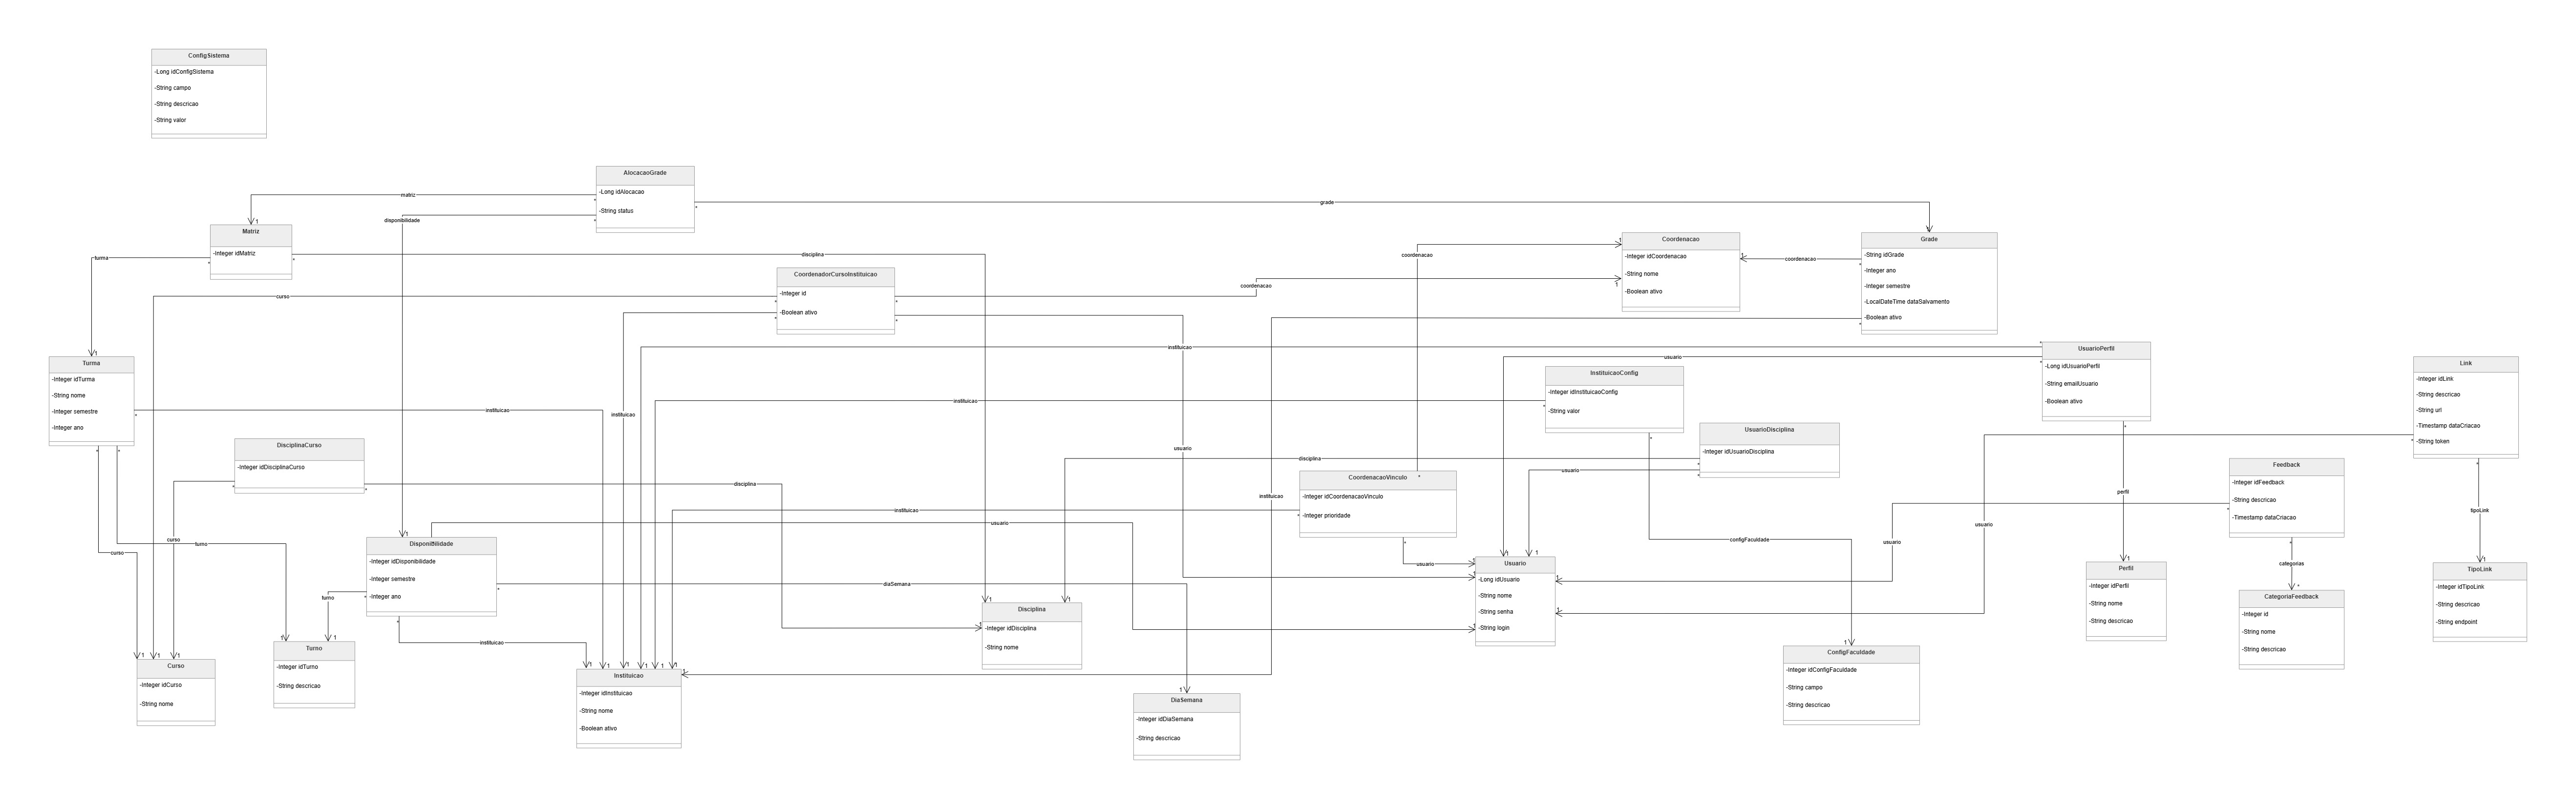
\includegraphics[width=\linewidth,height=0.9\textheight,keepaspectratio]{figuras/Figura_10_diagrama de classe.jpg}
\fonteautores
\end{figure}
\end{landscape}

\subsection{Especificação das Classes}
\label{subsec:4.3.2}

As tabelas a seguir descrevem os atributos, tipos de dados, visibilidade e semântica de cada classe identificada no modelo orientado a objetos do IGRIS, servindo como referência para a implementação das entidades de domínio.

% Tabela 64
\vspace{\baselineskip}

\Needspace{0.32\textheight}
\begin{longtable}{|L{3.5cm}|L{3.5cm}|L{3.5cm}|L{3.5cm}|}
\caption{Especificação da Classe: Instituicao} \\
\hline
\textbf{Elemento} & \textbf{Tipo/Assinatura} & \textbf{Visibilidade} & \textbf{Descrição} \\
\hline
\endfirsthead
\hline
\textbf{Elemento} & \textbf{Tipo/Assinatura} & \textbf{Visibilidade} & \textbf{Descrição} \\
\hline
\endhead
idInstituicao & int & private & Identificador único da instituição. \\
\hline
nome & String & private & Nome oficial da instituição. \\
\hline
ativo & boolean & private & Indicador se a instituição está ativa no sistema. \\
\hline
\end{longtable}

\fonteautores

% Tabela 65
\vspace{\baselineskip}

\Needspace{0.32\textheight}
\begin{longtable}{|L{3.5cm}|L{3.5cm}|L{3.5cm}|L{3.5cm}|}
\caption{Especificação da Classe: Coordenacao} \\
\hline
\textbf{Elemento} & \textbf{Tipo/Assinatura} & \textbf{Visibilidade} & \textbf{Descrição} \\
\hline
\endfirsthead
\hline
\textbf{Elemento} & \textbf{Tipo/Assinatura} & \textbf{Visibilidade} & \textbf{Descrição} \\
\hline
\endhead
idCoordenacao & int & private & Identificador da coordenação. \\
\hline
nome & String & private & Nome da coordenação (ex.: Engenharia de Software). \\
\hline
ativo & boolean & private & Indica se a coordenação está ativa. \\
\hline
instituicao & Instituicao & private & Instituição a que a coordenação pertence. \\
\hline
\end{longtable}

\fonteautores

% Tabela 66
\vspace{\baselineskip}

\Needspace{0.32\textheight}
\begin{longtable}{|L{3.5cm}|L{3.5cm}|L{3.5cm}|L{3.5cm}|}
\caption{Especificação da Classe: CoordenadorCursoInstituicao} \\
\hline
\textbf{Elemento} & \textbf{Tipo/Assinatura} & \textbf{Visibilidade} & \textbf{Descrição} \\
\hline
\endfirsthead
\hline
\textbf{Elemento} & \textbf{Tipo/Assinatura} & \textbf{Visibilidade} & \textbf{Descrição} \\
\hline
\endhead
idCoordenadorCurso & int & private & Identificador do vínculo do coordenador ao curso/instituição. \\
\hline
coordenacao & Coordenacao & private & Coordenação associada. \\
\hline
usuario & Usuario & private & Usuário que atua como coordenador. \\
\hline
instituicao & Instituicao & private & Instituição do vínculo. \\
\hline
curso & Curso & private & Curso coordenado. \\
\hline
\end{longtable}

\fonteautores

% Tabela 67
\vspace{\baselineskip}

\Needspace{0.32\textheight}
\begin{longtable}{|L{3.5cm}|L{3.5cm}|L{3.5cm}|L{3.5cm}|}
\caption{Especificação da Classe: CoordenacaoVinculo} \\
\hline
\textbf{Elemento} & \textbf{Tipo/Assinatura} & \textbf{Visibilidade} & \textbf{Descrição} \\
\hline
\endfirsthead
\hline
\textbf{Elemento} & \textbf{Tipo/Assinatura} & \textbf{Visibilidade} & \textbf{Descrição} \\
\hline
\endhead
usuario & Usuario & private & Usuário vinculado à coordenação. \\
\hline
coordenacao & Coordenacao & private & Coordenação vinculada. \\
\hline
instituicao & Instituicao & private & Instituição do vínculo. \\
\hline
prioridade & int & private & Prioridade do vínculo, usada para resolução de conflitos. \\
\hline
\end{longtable}

\fonteautores

% Tabela 68
\vspace{\baselineskip}

\Needspace{0.32\textheight}
\begin{longtable}{|L{3.5cm}|L{3.5cm}|L{3.5cm}|L{3.5cm}|}
\caption{Especificação da Classe: Curso} \\
\hline
\textbf{Elemento} & \textbf{Tipo/Assinatura} & \textbf{Visibilidade} & \textbf{Descrição} \\
\hline
\endfirsthead
\hline
\textbf{Elemento} & \textbf{Tipo/Assinatura} & \textbf{Visibilidade} & \textbf{Descrição} \\
\hline
\endhead
idCurso & int & private & Identificador do curso. \\
\hline
nome & String & private & Nome do curso (ex.: Ciência da Computação). \\
\hline
\end{longtable}

\fonteautores

% Tabela 69
\vspace{\baselineskip}

\Needspace{0.32\textheight}
\begin{longtable}{|L{3.5cm}|L{3.5cm}|L{3.5cm}|L{3.5cm}|}
\caption{Especificação da Classe: Disciplina} \\
\hline
\textbf{Elemento} & \textbf{Tipo/Assinatura} & \textbf{Visibilidade} & \textbf{Descrição} \\
\hline
\endfirsthead
\hline
\textbf{Elemento} & \textbf{Tipo/Assinatura} & \textbf{Visibilidade} & \textbf{Descrição} \\
\hline
\endhead
idDisciplina & int & private & Identificador da disciplina. \\
\hline
nome & String & private & Nome da disciplina. \\
\hline
\end{longtable}

\fonteautores

% Tabela 70
\vspace{\baselineskip}

\Needspace{0.32\textheight}
\begin{longtable}{|L{3.5cm}|L{3.5cm}|L{3.5cm}|L{3.5cm}|}
\caption{Especificação da Classe: DisciplinaCurso} \\
\hline
\textbf{Elemento} & \textbf{Tipo/Assinatura} & \textbf{Visibilidade} & \textbf{Descrição} \\
\hline
\endfirsthead
\hline
\textbf{Elemento} & \textbf{Tipo/Assinatura} & \textbf{Visibilidade} & \textbf{Descrição} \\
\hline
\endhead
idDisciplinaCurso & int & private & Identificador da associação disciplina-curso. \\
\hline
curso & Curso & private & Curso ao qual a disciplina pertence. \\
\hline
disciplina & Disciplina & private & Disciplina associada. \\
\hline
semestre & int & private & Semestre previsto na matriz curricular (quando aplicável). \\
\hline
\end{longtable}

\fonteautores

% Tabela 71
\vspace{\baselineskip}

\Needspace{0.32\textheight}
\begin{longtable}{|L{3.5cm}|L{3.5cm}|L{3.5cm}|L{3.5cm}|}
\caption{Especificação da Classe: Turma} \\
\hline
\textbf{Elemento} & \textbf{Tipo/Assinatura} & \textbf{Visibilidade} & \textbf{Descrição} \\
\hline
\endfirsthead
\hline
\textbf{Elemento} & \textbf{Tipo/Assinatura} & \textbf{Visibilidade} & \textbf{Descrição} \\
\hline
\endhead
idTurma & int & private & Identificador da turma. \\
\hline
nome & String & private & Nome/código da turma. \\
\hline
semestre & int & private & Semestre da oferta. \\
\hline
ano & int & private & Ano letivo. \\
\hline
id\_curso & int & private & Curso ao qual a turma pertence. \\
\hline
id\_turno & int & private & Turno (manhã/tarde/noite) da turma. \\
\hline
id\_instituicao & int & private & Instituição responsável. \\
\hline
\end{longtable}

\fonteautores

% Tabela 72
\vspace{\baselineskip}

\Needspace{0.32\textheight}
\begin{longtable}{|L{3.5cm}|L{3.5cm}|L{3.5cm}|L{3.5cm}|}
\caption{Especificação da Classe: Matriz} \\
\hline
\textbf{Elemento} & \textbf{Tipo/Assinatura} & \textbf{Visibilidade} & \textbf{Descrição} \\
\hline
\endfirsthead
\hline
\textbf{Elemento} & \textbf{Tipo/Assinatura} & \textbf{Visibilidade} & \textbf{Descrição} \\
\hline
\endhead
idMatriz & int & private & Identificador da matriz (grade curricular associada a uma turma/curso). \\
\hline
id\_turma & int & private & Turma relacionada à matriz. \\
\hline
id\_disciplina & int & private & Disciplina pertencente à matriz curricular. \\
\hline
semestre & int & private & Semestre em que a disciplina é prevista. \\
\hline
\end{longtable}

\fonteautores

% Tabela 73
\vspace{\baselineskip}

\Needspace{0.32\textheight}
\begin{longtable}{|L{3.5cm}|L{3.5cm}|L{3.5cm}|L{3.5cm}|}
\caption{Especificação da Classe: Usuario} \\
\hline
\textbf{Elemento} & \textbf{Tipo/Assinatura} & \textbf{Visibilidade} & \textbf{Descrição} \\
\hline
\endfirsthead
\hline
\textbf{Elemento} & \textbf{Tipo/Assinatura} & \textbf{Visibilidade} & \textbf{Descrição} \\
\hline
\endhead
idUsuario & int & private & Identificador único do usuário. \\
\hline
login & String & private & Login do usuário (único). \\
\hline
nome & String & private & Nome completo do usuário. \\
\hline
senha & String & private & Senha para autenticação (armazenada de forma segura). \\
\hline
email & String & private & E-mail de contato do usuário. \\
\hline
\end{longtable}

\fonteautores

% Tabela 74
\vspace{\baselineskip}

\Needspace{0.32\textheight}
\begin{longtable}{|L{3.5cm}|L{3.5cm}|L{3.5cm}|L{3.5cm}|}
\caption{Especificação da Classe: Perfil} \\
\hline
\textbf{Elemento} & \textbf{Tipo/Assinatura} & \textbf{Visibilidade} & \textbf{Descrição} \\
\hline
\endfirsthead
\hline
\textbf{Elemento} & \textbf{Tipo/Assinatura} & \textbf{Visibilidade} & \textbf{Descrição} \\
\hline
\endhead
idPerfil & int & private & Identificador do perfil (papel). \\
\hline
nome & String & private & Nome do perfil (ex.: Coordenador, Professor, Administrador). \\
\hline
\end{longtable}

\fonteautores

% Tabela 75
\vspace{\baselineskip}

\Needspace{0.32\textheight}
\begin{longtable}{|L{3.5cm}|L{3.5cm}|L{3.5cm}|L{3.5cm}|}
\caption{Especificação da Classe: UsuarioPerfil} \\
\hline
\textbf{Elemento} & \textbf{Tipo/Assinatura} & \textbf{Visibilidade} & \textbf{Descrição} \\
\hline
\endfirsthead
\hline
\textbf{Elemento} & \textbf{Tipo/Assinatura} & \textbf{Visibilidade} & \textbf{Descrição} \\
\hline
\endhead
idUsuarioPerfil & int & private & Identificador do vínculo entre usuário e perfil. \\
\hline
id\_usuario & int & private & Usuário associado. \\
\hline
id\_perfil & int & private & Perfil do usuário. \\
\hline
id\_instituicao & int & private & Instituição onde o perfil vale. \\
\hline
email & String & private & E-mail institucional ou contato do vínculo. \\
\hline
ativo & boolean & private & Indica se o vínculo/perfil está ativo. \\
\hline
\end{longtable}

\fonteautores

% Tabela 76
\vspace{\baselineskip}

\Needspace{0.32\textheight}
\begin{longtable}{|L{3.5cm}|L{3.5cm}|L{3.5cm}|L{3.5cm}|}
\caption{Especificação da Classe: UsuarioDisciplina} \\
\hline
\textbf{Elemento} & \textbf{Tipo/Assinatura} & \textbf{Visibilidade} & \textbf{Descrição} \\
\hline
\endfirsthead
\hline
\textbf{Elemento} & \textbf{Tipo/Assinatura} & \textbf{Visibilidade} & \textbf{Descrição} \\
\hline
\endhead
idUsuarioDisciplina & int & private & Identificador da associação usuário-disciplina. \\
\hline
id\_usuario & int & private & Professor/usuário apto a lecionar a disciplina. \\
\hline
id\_disciplina & int & private & Disciplina associada. \\
\hline
ano & int & private & Ano de referência da aptidão. \\
\hline
semestre & int & private & Semestre de referência da aptidão. \\
\hline
\end{longtable}

\fonteautores

% Tabela 77
\vspace{\baselineskip}

\Needspace{0.32\textheight}
\begin{longtable}{|L{3.5cm}|L{3.5cm}|L{3.5cm}|L{3.5cm}|}
\caption{Especificação da Classe: Disponibilidade} \\
\hline
\textbf{Elemento} & \textbf{Tipo/Assinatura} & \textbf{Visibilidade} & \textbf{Descrição} \\
\hline
\endfirsthead
\hline
\textbf{Elemento} & \textbf{Tipo/Assinatura} & \textbf{Visibilidade} & \textbf{Descrição} \\
\hline
\endhead
idDisponibilidade & int & private & Identificador da disponibilidade cadastrada. \\
\hline
semestre & int & private & Semestre a que a disponibilidade se aplica. \\
\hline
ano & int & private & Ano letivo da disponibilidade. \\
\hline
diaSemana & DiaSemana & private & Dia da semana referente. \\
\hline
usuario & Usuario & private & Usuário que registra a disponibilidade (professor). \\
\hline
turno & Turno & private & Turno disponível. \\
\hline
turma & Turma & private & Turma relacionada, quando aplicável. \\
\hline
instituicao & Instituicao & private & Instituição do registro. \\
\hline
\end{longtable}

\fonteautores

% Tabela 78
\vspace{\baselineskip}

\Needspace{0.32\textheight}
\begin{longtable}{|L{3.5cm}|L{3.5cm}|L{3.5cm}|L{3.5cm}|}
\caption{Especificação da Classe: Turno} \\
\hline
\textbf{Elemento} & \textbf{Tipo/Assinatura} & \textbf{Visibilidade} & \textbf{Descrição} \\
\hline
\endfirsthead
\hline
\textbf{Elemento} & \textbf{Tipo/Assinatura} & \textbf{Visibilidade} & \textbf{Descrição} \\
\hline
\endhead
idTurno & int & private & Identificador do turno. \\
\hline
descricao & String & private & Descrição do turno (Manhã/Tarde/Noite). \\
\hline
ativo & boolean & private & Indica se o turno está ativo no catálogo. \\
\hline
\end{longtable}

\fonteautores

% Tabela 79
\vspace{\baselineskip}

\Needspace{0.32\textheight}
\begin{longtable}{|L{3.5cm}|L{3.5cm}|L{3.5cm}|L{3.5cm}|}
\caption{Especificação da Classe: DiaSemana} \\
\hline
\textbf{Elemento} & \textbf{Tipo/Assinatura} & \textbf{Visibilidade} & \textbf{Descrição} \\
\hline
\endfirsthead
\hline
\textbf{Elemento} & \textbf{Tipo/Assinatura} & \textbf{Visibilidade} & \textbf{Descrição} \\
\hline
\endhead
idDiaSemana & int & private & Identificador do dia da semana. \\
\hline
descricao & String & private & Nome do dia (Segunda, Terça, ...). \\
\hline
ativo & boolean & private & Indica se o dia está habilitado no calendário. \\
\hline
\end{longtable}

\fonteautores

% Tabela 80
\vspace{\baselineskip}

\Needspace{0.32\textheight}
\begin{longtable}{|L{3.5cm}|L{3.5cm}|L{3.5cm}|L{3.5cm}|}
\caption{Especificação da Classe: AlocacaoGrade} \\
\hline
\textbf{Elemento} & \textbf{Tipo/Assinatura} & \textbf{Visibilidade} & \textbf{Descrição} \\
\hline
\endfirsthead
\hline
\textbf{Elemento} & \textbf{Tipo/Assinatura} & \textbf{Visibilidade} & \textbf{Descrição} \\
\hline
\endhead
idLinha & int & private & Identificador da linha de alocação na grade. \\
\hline
usuario & Usuario & private & Professor alocado. \\
\hline
disciplina & Disciplina & private & Disciplina alocada. \\
\hline
diaSemana & DiaSemana & private & Dia da semana da aula. \\
\hline
turno & Turno & private & Turno/hora da alocação. \\
\hline
turma & Turma & private & Turma alocada. \\
\hline
grade & Grade & private & Referência à grade onde a alocação pertence. \\
\hline
\end{longtable}

\fonteautores

% Tabela 81
\vspace{\baselineskip}

\Needspace{0.32\textheight}
\begin{longtable}{|L{3.5cm}|L{3.5cm}|L{3.5cm}|L{3.5cm}|}
\caption{Especificação da Classe: Grade} \\
\hline
\textbf{Elemento} & \textbf{Tipo/Assinatura} & \textbf{Visibilidade} & \textbf{Descrição} \\
\hline
\endfirsthead
\hline
\textbf{Elemento} & \textbf{Tipo/Assinatura} & \textbf{Visibilidade} & \textbf{Descrição} \\
\hline
\endhead
idGrade & String & private & Identificador da grade (pode ser GUID). \\
\hline
id\_usuario & Usuario & private & Usuário que gerou a grade (coordenador/sistema). \\
\hline
ano & int & private & Ano letivo da grade. \\
\hline
semestre & int & private & Semestre da grade. \\
\hline
dataGeracao & date & private & Timestamp da geração da grade. \\
\hline
\end{longtable}

\fonteautores

% Tabela 82
\vspace{\baselineskip}

\Needspace{0.32\textheight}
\begin{longtable}{|L{3.5cm}|L{3.5cm}|L{3.5cm}|L{3.5cm}|}
\caption{Especificação da Classe: Links} \\
\hline
\textbf{Elemento} & \textbf{Tipo/Assinatura} & \textbf{Visibilidade} & \textbf{Descrição} \\
\hline
\endfirsthead
\hline
\textbf{Elemento} & \textbf{Tipo/Assinatura} & \textbf{Visibilidade} & \textbf{Descrição} \\
\hline
\endhead
idLink & int & private & Identificador do link/recurso. \\
\hline
url & String & private & Endereço do recurso/link. \\
\hline
dtGerada & date & private & Data de geração do link/recurso. \\
\hline
horas & int & private & Tempo associado (quando aplicável). \\
\hline
tipoLink & TipoLink & private & Tipo do link (categoria). \\
\hline
usuario & Usuario & private & Usuário que criou/usa o link. \\
\hline
\end{longtable}

\fonteautores

% Tabela 83
\vspace{\baselineskip}

\Needspace{0.32\textheight}
\begin{longtable}{|L{3.5cm}|L{3.5cm}|L{3.5cm}|L{3.5cm}|}
\caption{Especificação da Classe: TipoLink} \\
\hline
\textbf{Elemento} & \textbf{Tipo/Assinatura} & \textbf{Visibilidade} & \textbf{Descrição} \\
\hline
\endfirsthead
\hline
\textbf{Elemento} & \textbf{Tipo/Assinatura} & \textbf{Visibilidade} & \textbf{Descrição} \\
\hline
\endhead
idTipoLink & int & private & Identificador do tipo de link. \\
\hline
nome & String & private & Nome do tipo de link. \\
\hline
descricao & String & private & Descrição do propósito do link. \\
\hline
\end{longtable}

\fonteautores

\section{Modelagem de Dados}
\label{sec:4.4}

A modelagem de dados do IGRIS foi projetada com foco na integridade referencial e na otimização de consultas, utilizando o Sistema Gerenciador de Banco de Dados relacional PostgreSQL 15. Conforme \citeonline{silberschatz2001}, o modelo relacional oferece mecanismos robustos para garantir a integridade e a consistência dos dados, fundamentais para aplicações críticas que envolvem múltiplos módulos interdependentes.

\subsection{Diagrama Entidade-Relacionamento}
\label{subsec:4.4.1}

Devido à complexidade do domínio e ao número de tabelas envolvidas, o modelo de dados é apresentado em quatro perspectivas complementares: uma visão geral consolidada e três recortes temáticos.

A Figura do DER Completo apresenta uma visão panorâmica de todas as tabelas e seus relacionamentos, permitindo compreender a estrutura global do banco de dados.

O módulo acadêmico abrange as entidades centrais do negócio: curso, turma, disciplina, disciplina\_curso, matriz, usuario\_disciplina, coordenador\_curso\_instituicao, dia\_semana, turno, disponibilidade, alocacao\_grade e grade. A entidade alocacao\_grade é o coração do sistema, registrando cada alocação gerada pelo algoritmo genético ao vincular uma matriz, uma disponibilidade e uma grade.

O módulo de controle de acesso consolida as entidades responsáveis pela segurança e autenticação: usuario, perfil, usuario\_perfil, link, tipo\_link, coordenacao, coordenacao\_vinculo, feedback e categorias\_feedback. A tabela usuario\_perfil implementa o controle multi-perfil, permitindo que um mesmo usuário assuma diferentes papéis institucionais.

O módulo institucional representa a configuração das instituições: instituicao, config\_faculdade, instituicao\_config, config\_sistema e erros. Essas entidades permitem que cada instituição personalize seus parâmetros operacionais de forma independente, incluindo os hiperparâmetros do algoritmo genético armazenados em config\_sistema.

\begin{landscape}

\begin{figure}[H]
\centering
\caption{Diagrama de Entidade-Relacionamento: Módulo de Controle de Acesso}
\label{fig:der_acesso}
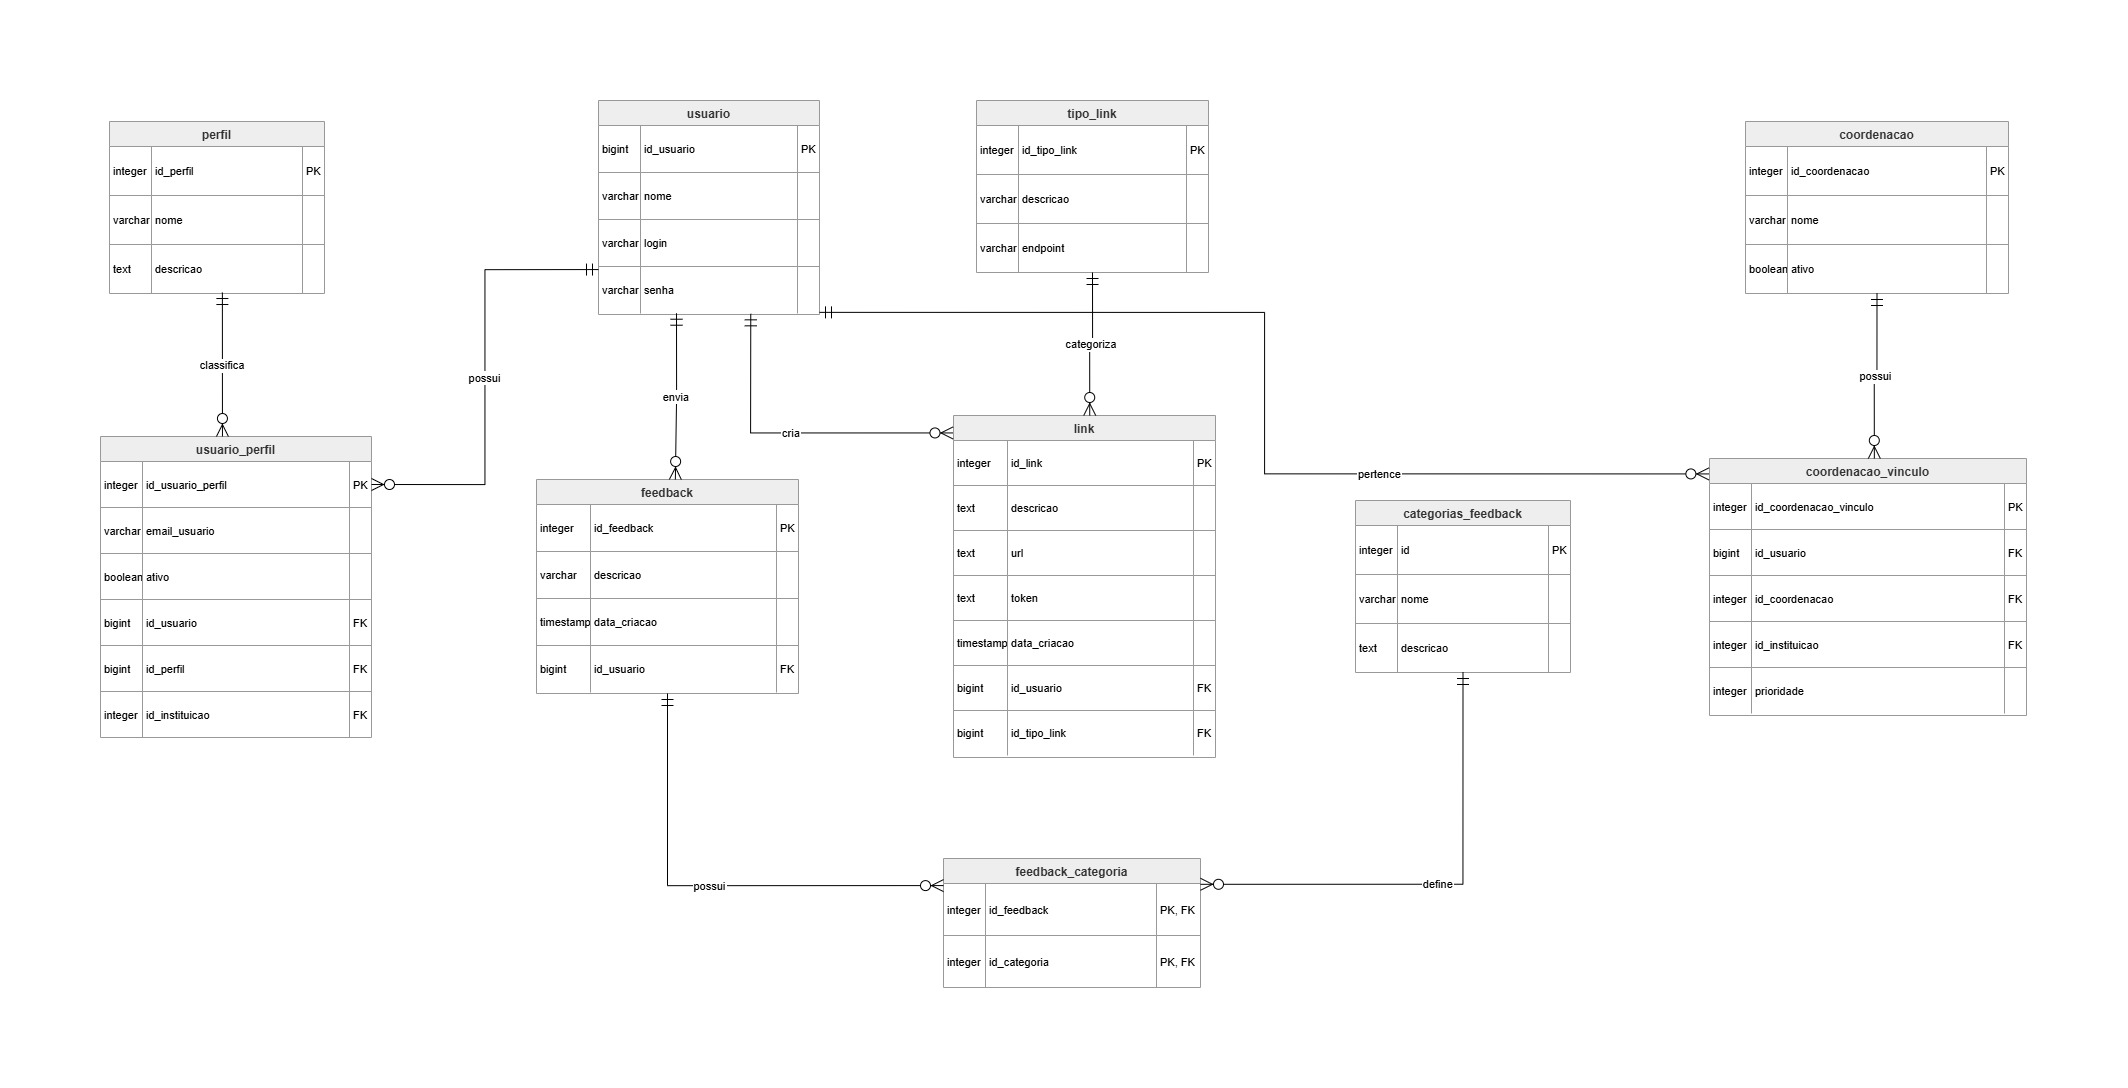
\includegraphics[width=\linewidth,height=0.9\textheight,keepaspectratio]{figuras/Figura_11_Diagrama ER_controle de acesso.jpg}
\fonteautores
\end{figure}

\newpage

\begin{figure}[H]
\centering
\caption{Diagrama de Entidade-Relacionamento: Módulo Acadêmico}
\label{fig:der_academico}
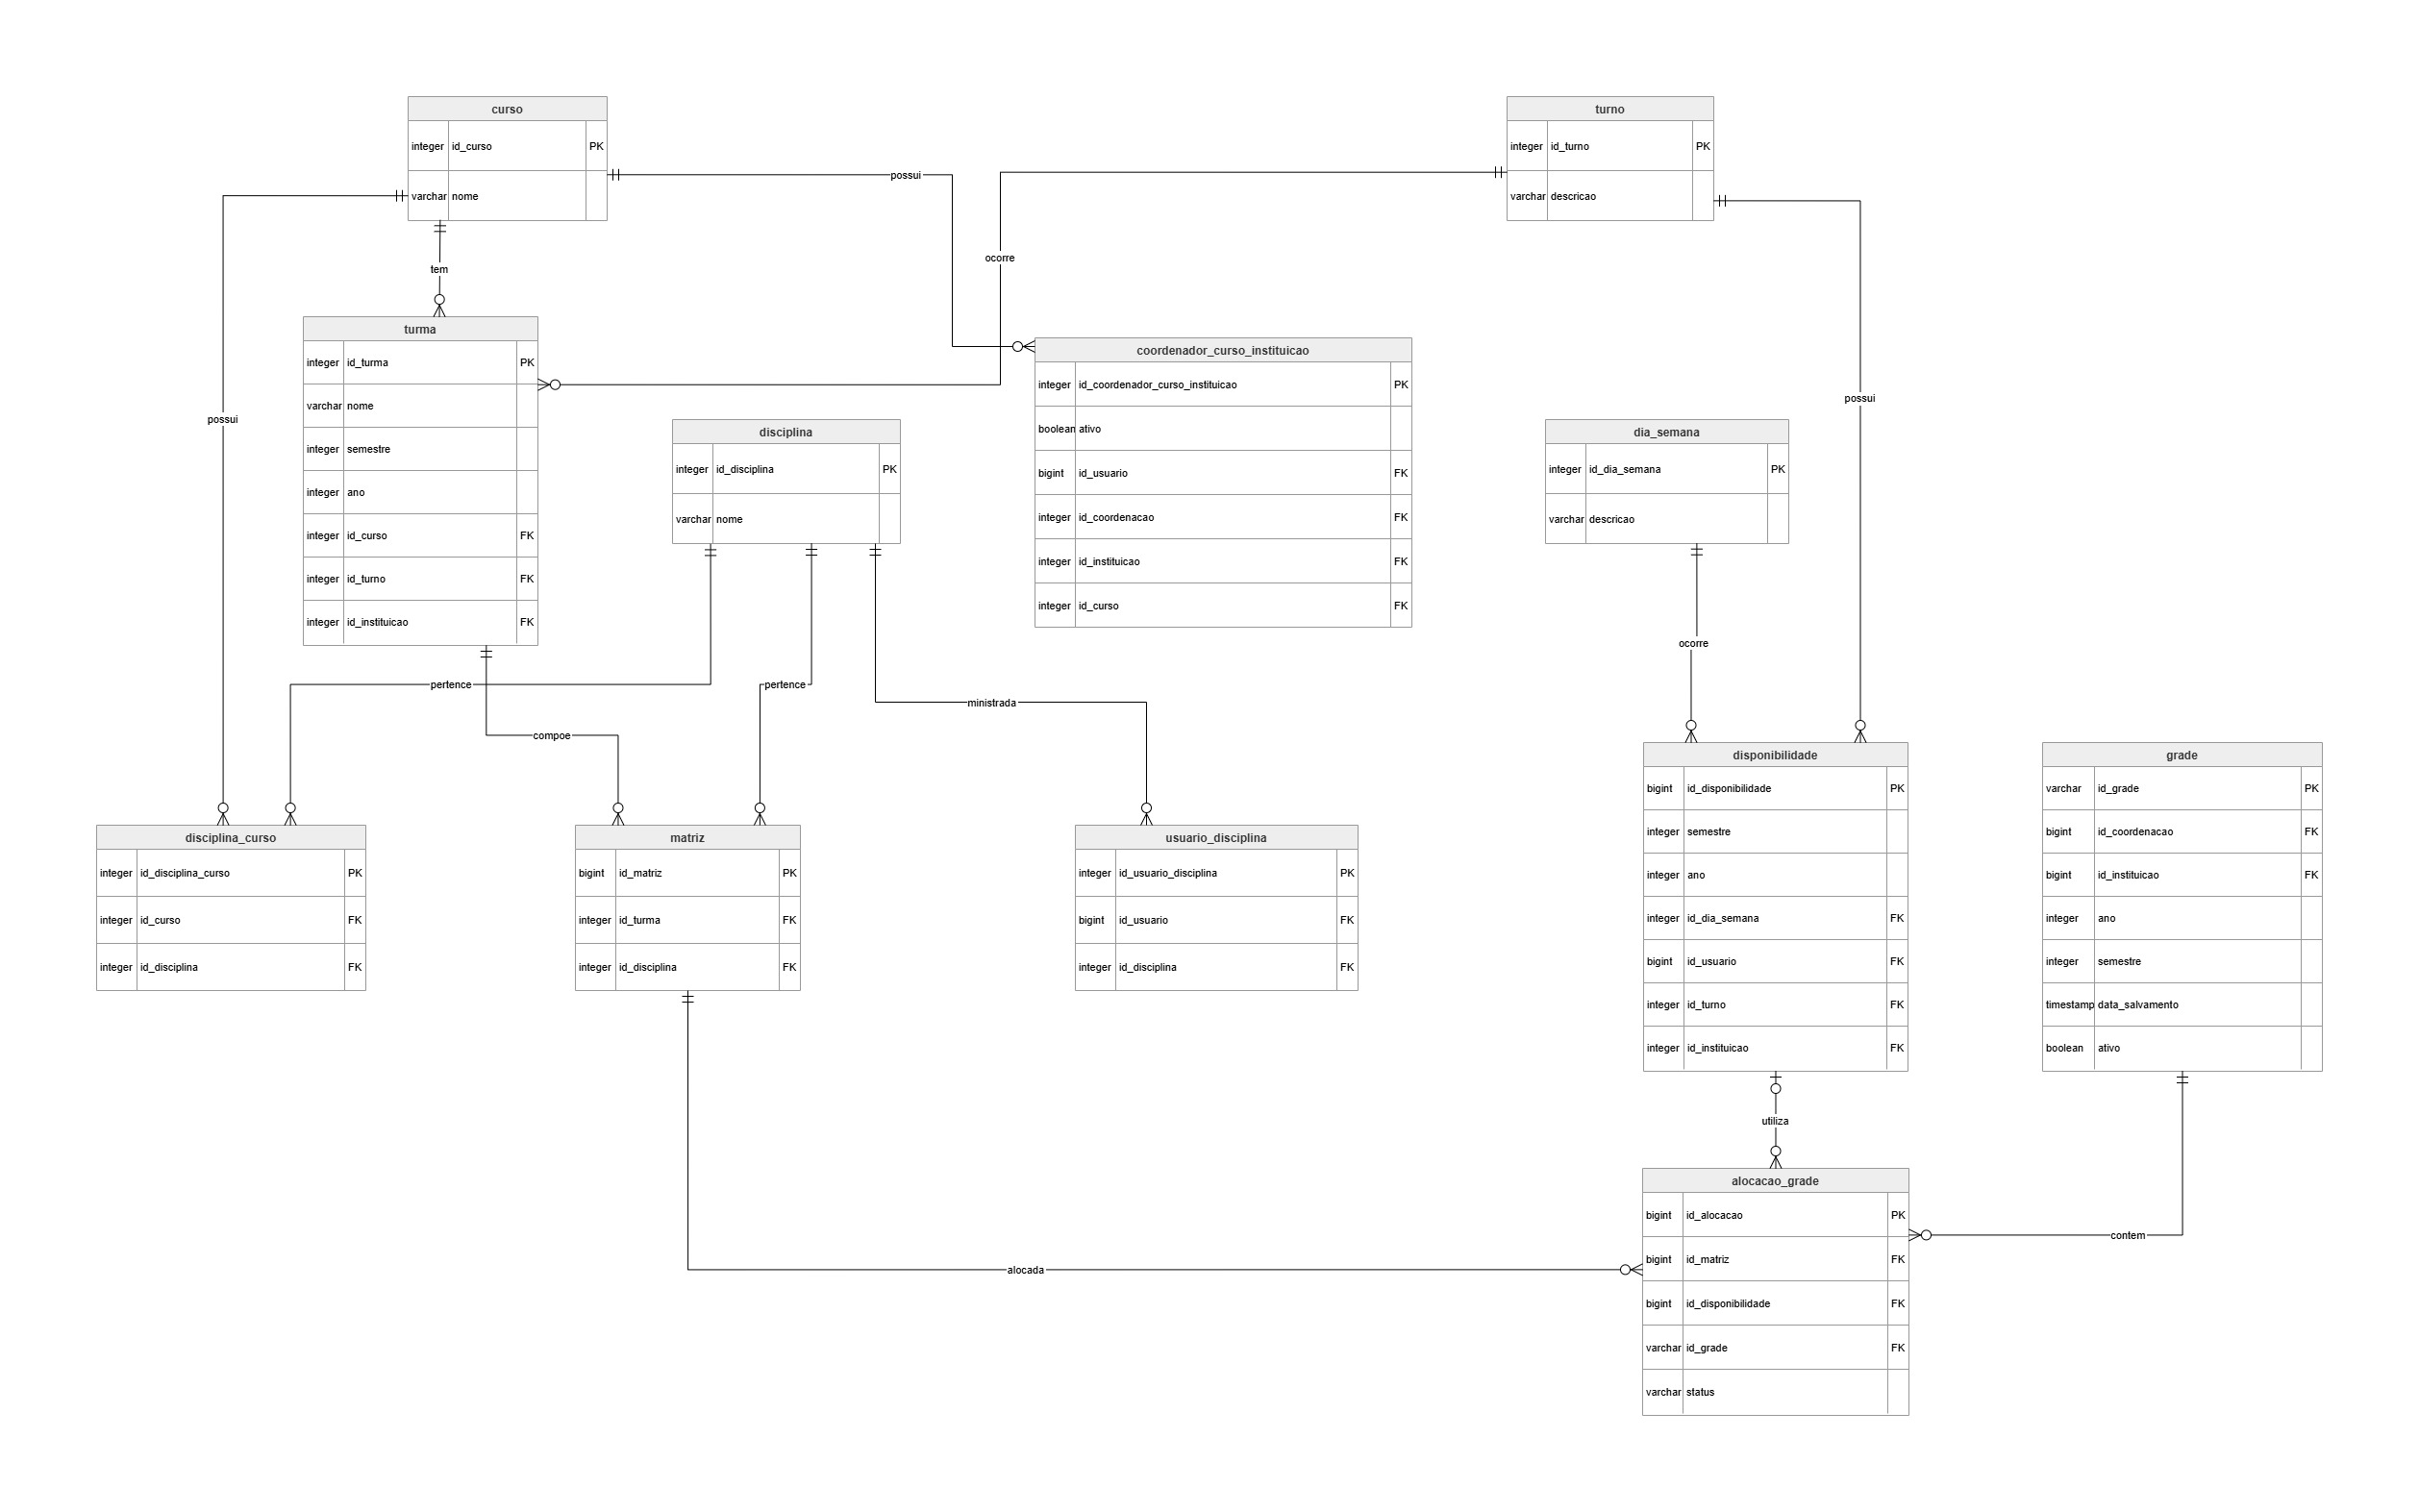
\includegraphics[width=\linewidth,height=0.9\textheight,keepaspectratio]{figuras/Figura_12_diagrama ER_academico.jpg}
\fonteautores
\end{figure}

\newpage

\begin{figure}[H]
\centering
\caption{Diagrama de Entidade-Relacionamento: Módulo Institucional}
\label{fig:der_institucional}
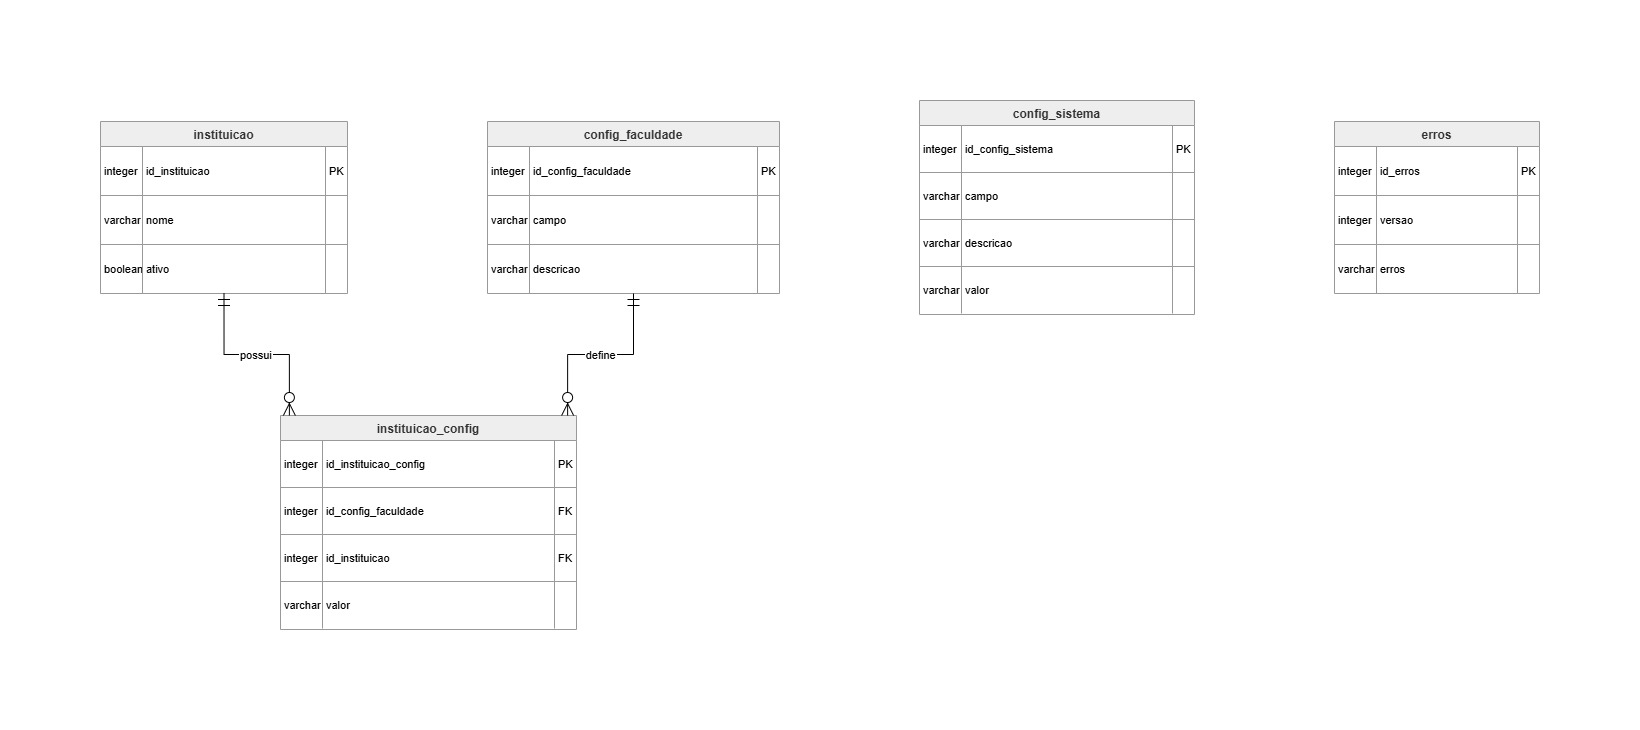
\includegraphics[width=\linewidth,height=0.9\textheight,keepaspectratio]{figuras/Figura_13_diagrama ER instituicao.jpg}
\fonteautores
\end{figure}

\end{landscape}

\begin{landscape}

\begin{figure}[H]
\centering
\caption{Diagrama de Entidade-Relacionamento Completo}
\label{fig:der_completo}
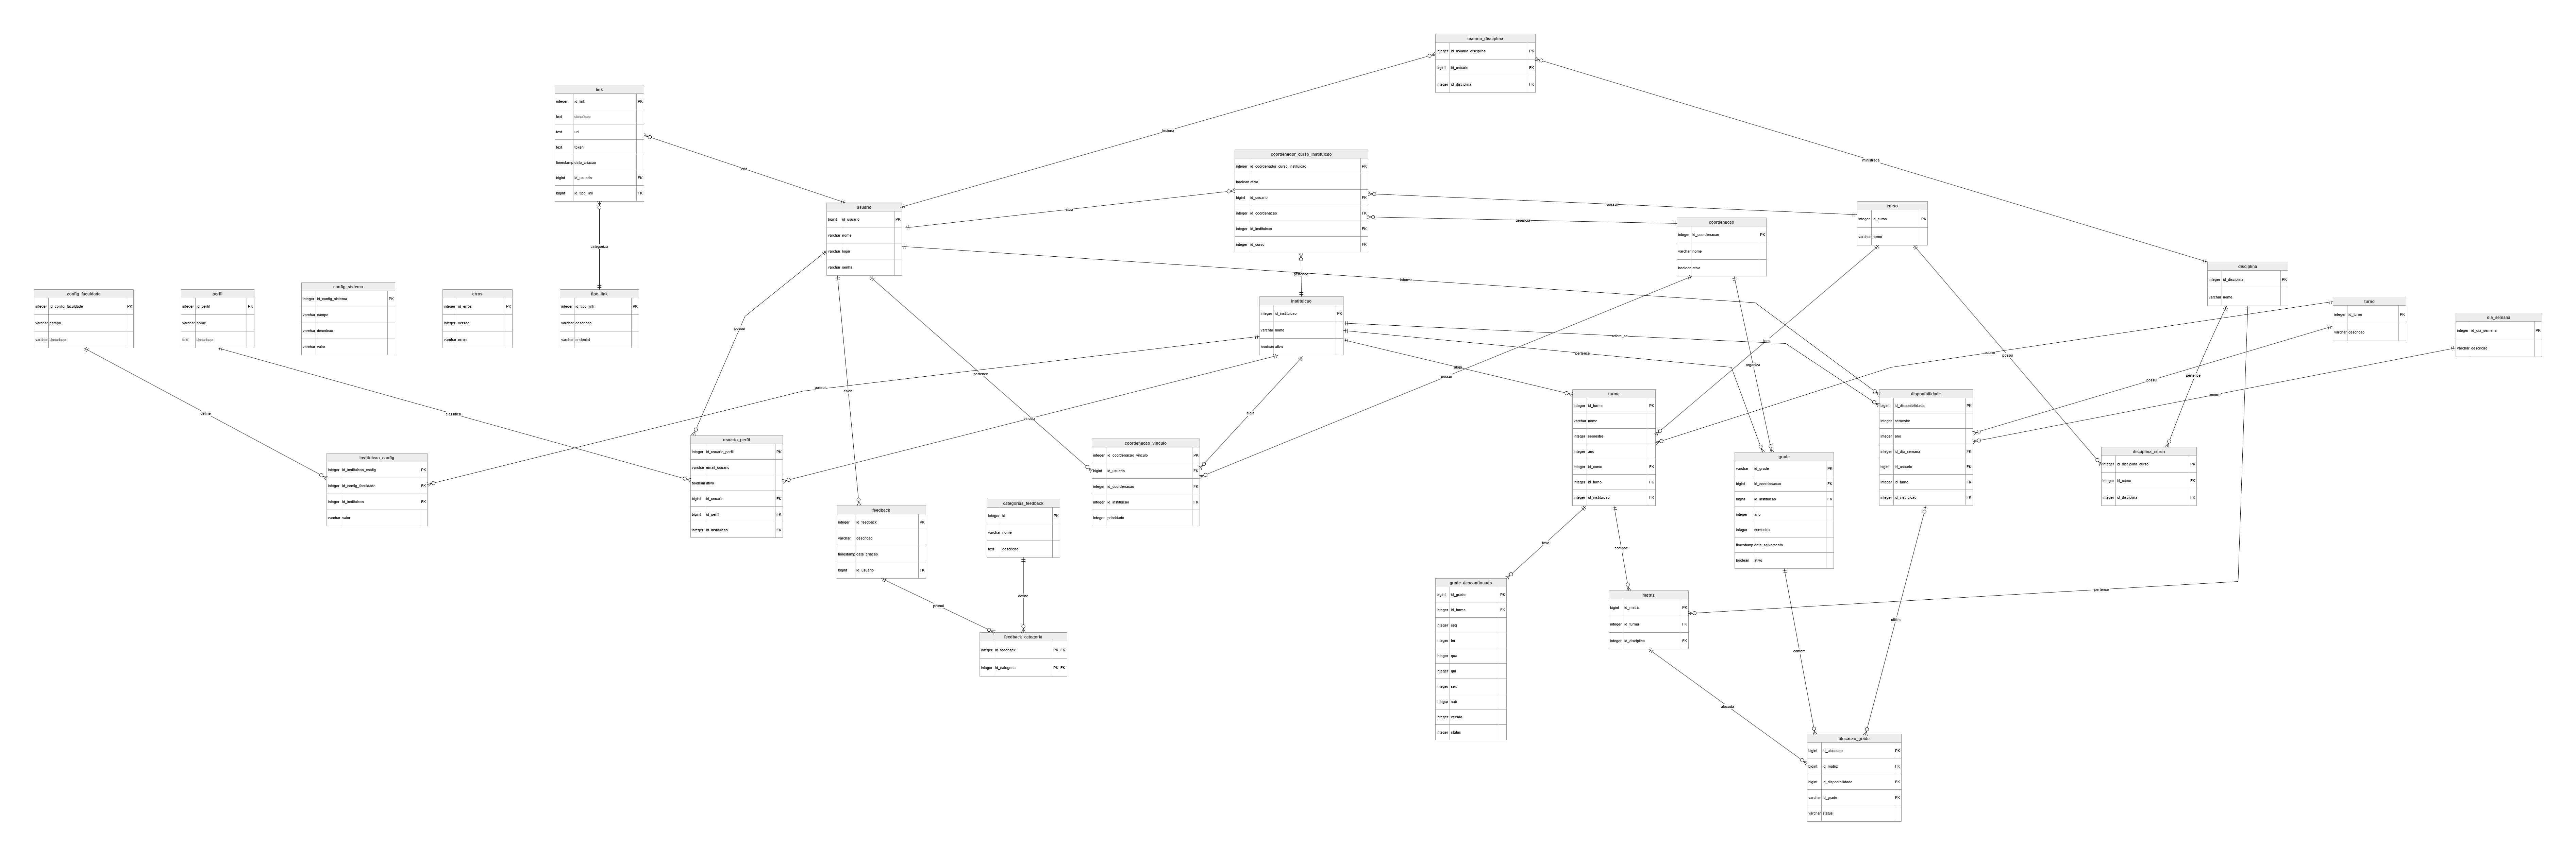
\includegraphics[width=\linewidth,height=\textheight,keepaspectratio]{figuras/Figura_14_diagrama ER completo.jpg}
\fonteautores
\end{figure}

\end{landscape}

\subsection{Dicionário de Dados}
\label{subsec:4.4.2}

\begingroup
\small
\sloppy
\setlength{\tabcolsep}{3pt}

O dicionário de dados complementa a representação gráfica do Modelo Entidade-Relacionamento, descrevendo a estrutura física das tabelas com tipos de dados, restrições de integridade e a semântica de cada atributo. Os Quadros de Tabela 37 a Tabela 63 apresentam a especificação completa das 27 tabelas do banco de dados do IGRIS.

% Tabela 37
\vspace{\baselineskip}

\Needspace{0.32\textheight}
\begin{longtable}{|L{5.2cm}|L{3.2cm}|L{2.4cm}|L{3.4cm}|}
\caption{instituicao} \\
\hline
\textbf{Variável} & \textbf{Tipo} & \textbf{Propriedades} & \textbf{Descrição} \\
\hline
\endfirsthead
\hline
\textbf{Variável} & \textbf{Tipo} & \textbf{Propriedades} & \textbf{Descrição} \\
\hline
\endhead
id\_instituicao & Integer (4 bytes) & PK & Código de identificação da tabela \\
\hline
nome & character varying (255) & NOT NULL & Nome da instituição de ensino \\
\hline
ativo & boolean (1 byte) & NOT NULL & Indica se a instituição está ativa no sistema \\
\hline
\end{longtable}

\fonteautores

% Tabela 38
\vspace{\baselineskip}

\Needspace{0.32\textheight}
\begin{longtable}{|L{5.2cm}|L{3.2cm}|L{2.4cm}|L{3.4cm}|}
\caption{config\_faculdade} \\
\hline
\textbf{Variável} & \textbf{Tipo} & \textbf{Propriedades} & \textbf{Descrição} \\
\hline
\endfirsthead
\hline
\textbf{Variável} & \textbf{Tipo} & \textbf{Propriedades} & \textbf{Descrição} \\
\hline
\endhead
id\_config\_faculdade & Integer (4 bytes) & PK & Código de identificação da tabela \\
\hline
campo & character varying (255) & NOT NULL & Nome identificador da configuração \\
\hline
descricao & character varying (255) & NULL & Descrição textual explicando a finalidade da configuração \\
\hline
\end{longtable}

\fonteautores

% Tabela 39
\vspace{\baselineskip}

\Needspace{0.32\textheight}
\begin{longtable}{|L{5.2cm}|L{3.2cm}|L{2.4cm}|L{3.4cm}|}
\caption{instituicao\_config} \\
\hline
\textbf{Variável} & \textbf{Tipo} & \textbf{Propriedades} & \textbf{Descrição} \\
\hline
\endfirsthead
\hline
\textbf{Variável} & \textbf{Tipo} & \textbf{Propriedades} & \textbf{Descrição} \\
\hline
\endhead
id\_instituicao\_config & Integer (4 bytes) & PK & Código de identificação da tabela \\
\hline
id\_config\_faculdade & Integer (4 bytes) & FK – config\_faculdade & Referência à configuração do catálogo \\
\hline
id\_instituicao & Integer (4 bytes) & FK – instituicao & Referência à instituição dona da configuração \\
\hline
valor & character varying (255) & NULL & Valor atribuído à configuração para esta instituição \\
\hline
\end{longtable}

\fonteautores

% Tabela 40
\vspace{\baselineskip}

\Needspace{0.32\textheight}
\begin{longtable}{|L{5.2cm}|L{3.2cm}|L{2.4cm}|L{3.4cm}|}
\caption{config\_sistema} \\
\hline
\textbf{Variável} & \textbf{Tipo} & \textbf{Propriedades} & \textbf{Descrição} \\
\hline
\endfirsthead
\hline
\textbf{Variável} & \textbf{Tipo} & \textbf{Propriedades} & \textbf{Descrição} \\
\hline
\endhead
id\_config\_sistema & Integer (4 bytes) & PK & Código de identificação da tabela \\
\hline
campo & character varying (255) & NOT NULL & Nome identificador do parâmetro (ex: TAMANHO\_POPULACAO) \\
\hline
descricao & character varying (255) & NULL & Descrição textual explicando o parâmetro \\
\hline
valor & character varying (255) & NULL & Valor atual do parâmetro \\
\hline
\end{longtable}

\fonteautores

% Tabela 41
\vspace{\baselineskip}

\Needspace{0.32\textheight}
\begin{longtable}{|L{5.2cm}|L{3.2cm}|L{2.4cm}|L{3.4cm}|}
\caption{erros} \\
\hline
\textbf{Variável} & \textbf{Tipo} & \textbf{Propriedades} & \textbf{Descrição} \\
\hline
\endfirsthead
\hline
\textbf{Variável} & \textbf{Tipo} & \textbf{Propriedades} & \textbf{Descrição} \\
\hline
\endhead
id\_erros & Integer (4 bytes) & PK & Código de identificação da tabela \\
\hline
versao & Integer (4 bytes) & NULL & Número da versão do sistema no momento do erro \\
\hline
erros & character varying (255) & NULL & Descrição textual do erro registrado \\
\hline
\end{longtable}

\fonteautores

% Tabela 42
\vspace{\baselineskip}

\Needspace{0.32\textheight}
\begin{longtable}{|L{5.2cm}|L{3.2cm}|L{2.4cm}|L{3.4cm}|}
\caption{usuario} \\
\hline
\textbf{Variável} & \textbf{Tipo} & \textbf{Propriedades} & \textbf{Descrição} \\
\hline
\endfirsthead
\hline
\textbf{Variável} & \textbf{Tipo} & \textbf{Propriedades} & \textbf{Descrição} \\
\hline
\endhead
id\_usuario & bigint (8 bytes) & PK & Código de identificação da tabela \\
\hline
nome & character varying (255) & NOT NULL & Nome completo do usuário \\
\hline
login & character varying (255) & NOT NULL, UNIQUE & Login único de acesso ao sistema \\
\hline
senha & character varying (255) & NOT NULL & Senha criptografada (BCrypt) do usuário \\
\hline
\end{longtable}

\fonteautores

% Tabela 43
\vspace{\baselineskip}

\Needspace{0.32\textheight}
\begin{longtable}{|L{5.2cm}|L{3.2cm}|L{2.4cm}|L{3.4cm}|}
\caption{perfil} \\
\hline
\textbf{Variável} & \textbf{Tipo} & \textbf{Propriedades} & \textbf{Descrição} \\
\hline
\endfirsthead
\hline
\textbf{Variável} & \textbf{Tipo} & \textbf{Propriedades} & \textbf{Descrição} \\
\hline
\endhead
id\_perfil & Integer (4 bytes) & PK & Código de identificação da tabela \\
\hline
nome & character varying (255) & NOT NULL & Nome do perfil de acesso \\
\hline
descricao & text (variável) & NULL & Descrição das permissões do perfil \\
\hline
\end{longtable}

\fonteautores

% Tabela 44
\vspace{\baselineskip}

\Needspace{0.32\textheight}
\begin{longtable}{|L{5.2cm}|L{3.2cm}|L{2.4cm}|L{3.4cm}|}
\caption{usuario\_perfil} \\
\hline
\textbf{Variável} & \textbf{Tipo} & \textbf{Propriedades} & \textbf{Descrição} \\
\hline
\endfirsthead
\hline
\textbf{Variável} & \textbf{Tipo} & \textbf{Propriedades} & \textbf{Descrição} \\
\hline
\endhead
id\_usuario\_perfil & Integer (4 bytes) & PK & Código de identificação da tabela \\
\hline
email\_usuario & character varying (255) & NULL & E-mail do usuário neste vínculo específico \\
\hline
ativo & boolean (1 byte) & NOT NULL & Indica se este vínculo de perfil está ativo \\
\hline
id\_usuario & bigint (8 bytes) & FK – usuario & Referência ao usuário \\
\hline
id\_perfil & bigint (8 bytes) & FK – perfil & Referência ao perfil de acesso \\
\hline
id\_instituicao & Integer (4 bytes) & FK – instituicao & Referência à instituição do vínculo \\
\hline
\end{longtable}

\fonteautores

% Tabela 45
\vspace{\baselineskip}

\Needspace{0.32\textheight}
\begin{longtable}{|L{5.2cm}|L{3.2cm}|L{2.4cm}|L{3.4cm}|}
\caption{tipo\_link} \\
\hline
\textbf{Variável} & \textbf{Tipo} & \textbf{Propriedades} & \textbf{Descrição} \\
\hline
\endfirsthead
\hline
\textbf{Variável} & \textbf{Tipo} & \textbf{Propriedades} & \textbf{Descrição} \\
\hline
\endhead
id\_tipo\_link & Integer (4 bytes) & PK & Código de identificação da tabela \\
\hline
descricao & character varying (255) & NOT NULL & Descrição do tipo de link \\
\hline
endpoint & character varying (255) & NULL & Rota/endpoint associado ao tipo de link \\
\hline
\end{longtable}

\fonteautores

% Tabela 46
\vspace{\baselineskip}

\Needspace{0.32\textheight}
\begin{longtable}{|L{5.2cm}|L{3.2cm}|L{2.4cm}|L{3.4cm}|}
\caption{link} \\
\hline
\textbf{Variável} & \textbf{Tipo} & \textbf{Propriedades} & \textbf{Descrição} \\
\hline
\endfirsthead
\hline
\textbf{Variável} & \textbf{Tipo} & \textbf{Propriedades} & \textbf{Descrição} \\
\hline
\endhead
id\_link & Integer (4 bytes) & PK & Código de identificação da tabela \\
\hline
descricao & text (variável) & NULL & Descrição ou finalidade do link gerado \\
\hline
url & text (variável) & NULL & URL completa do link gerado \\
\hline
token & text (variável) & NOT NULL & Token criptografado para validação do link \\
\hline
data\_criacao & timestamp (8 bytes) & NOT NULL & Data e hora da criação do link \\
\hline
id\_usuario & bigint (8 bytes) & FK – usuario & Referência ao usuário que criou o link \\
\hline
id\_tipo\_link & bigint (8 bytes) & FK – tipo\_link & Referência ao tipo de link \\
\hline
\end{longtable}

\fonteautores

% Tabela 47
\vspace{\baselineskip}

\Needspace{0.32\textheight}
\begin{longtable}{|L{5.2cm}|L{3.2cm}|L{2.4cm}|L{3.4cm}|}
\caption{feedback} \\
\hline
\textbf{Variável} & \textbf{Tipo} & \textbf{Propriedades} & \textbf{Descrição} \\
\hline
\endfirsthead
\hline
\textbf{Variável} & \textbf{Tipo} & \textbf{Propriedades} & \textbf{Descrição} \\
\hline
\endhead
id\_feedback & Integer (4 bytes) & PK & Código de identificação da tabela \\
\hline
descricao & character varying (255) & NOT NULL & Texto descritivo do feedback enviado \\
\hline
data\_criacao & timestamp (8 bytes) & NOT NULL & Data e hora do envio do feedback \\
\hline
id\_usuario & bigint (8 bytes) & FK – usuario & Referência ao usuário remetente \\
\hline
\end{longtable}

\fonteautores

% Tabela 48
\vspace{\baselineskip}

\Needspace{0.32\textheight}
\begin{longtable}{|L{5.2cm}|L{3.2cm}|L{2.4cm}|L{3.4cm}|}
\caption{categorias\_feedback} \\
\hline
\textbf{Variável} & \textbf{Tipo} & \textbf{Propriedades} & \textbf{Descrição} \\
\hline
\endfirsthead
\hline
\textbf{Variável} & \textbf{Tipo} & \textbf{Propriedades} & \textbf{Descrição} \\
\hline
\endhead
id & Integer (4 bytes) & PK & Código de identificação da tabela \\
\hline
nome & character varying (255) & NOT NULL & Nome da categoria \\
\hline
descricao & text (variável) & NULL & Descrição detalhada da categoria \\
\hline
\end{longtable}

\fonteautores

% Tabela 49
\vspace{\baselineskip}

\Needspace{0.32\textheight}
\begin{longtable}{|L{5.2cm}|L{3.2cm}|L{2.4cm}|L{3.4cm}|}
\caption{feedback\_categoria} \\
\hline
\textbf{Variável} & \textbf{Tipo} & \textbf{Propriedades} & \textbf{Descrição} \\
\hline
\endfirsthead
\hline
\textbf{Variável} & \textbf{Tipo} & \textbf{Propriedades} & \textbf{Descrição} \\
\hline
\endhead
id\_feedback & Integer (4 bytes) & PK, FK – feedback & Referência ao feedback \\
\hline
id\_categoria & Integer (4 bytes) & PK, FK – categorias\_feedback & Referência à categoria do feedback \\
\hline
\end{longtable}

\fonteautores

% Tabela 50
\vspace{\baselineskip}

\Needspace{0.32\textheight}
\begin{longtable}{|L{5.2cm}|L{3.2cm}|L{2.4cm}|L{3.4cm}|}
\caption{coordenacao} \\
\hline
\textbf{Variável} & \textbf{Tipo} & \textbf{Propriedades} & \textbf{Descrição} \\
\hline
\endfirsthead
\hline
\textbf{Variável} & \textbf{Tipo} & \textbf{Propriedades} & \textbf{Descrição} \\
\hline
\endhead
id\_coordenacao & Integer (4 bytes) & PK & Código de identificação da tabela \\
\hline
nome & character varying (255) & NOT NULL & Nome da coordenação/departamento \\
\hline
ativo & boolean (1 byte) & NOT NULL & Indica se a coordenação está ativa \\
\hline
\end{longtable}

\fonteautores

% Tabela 51
\vspace{\baselineskip}

\Needspace{0.32\textheight}
\begin{longtable}{|L{5.2cm}|L{3.2cm}|L{2.4cm}|L{3.4cm}|}
\caption{coordenacao\_vinculo} \\
\hline
\textbf{Variável} & \textbf{Tipo} & \textbf{Propriedades} & \textbf{Descrição} \\
\hline
\endfirsthead
\hline
\textbf{Variável} & \textbf{Tipo} & \textbf{Propriedades} & \textbf{Descrição} \\
\hline
\endhead
id\_coordenacao\_vinculo & Integer (4 bytes) & PK & Código de identificação da tabela \\
\hline
id\_usuario & bigint (8 bytes) & FK – usuario & Referência ao usuário (coordenador) \\
\hline
id\_coordenacao & Integer (4 bytes) & FK – coordenacao & Referência à coordenação \\
\hline
id\_instituicao & Integer (4 bytes) & FK – instituicao & Referência à instituição \\
\hline
prioridade & Integer (4 bytes) & NULL & Nível de prioridade do vínculo \\
\hline
\end{longtable}

\fonteautores

% Tabela 52
\vspace{\baselineskip}

\Needspace{0.32\textheight}
\begin{longtable}{|L{5.2cm}|L{3.2cm}|L{2.4cm}|L{3.4cm}|}
\caption{curso} \\
\hline
\textbf{Variável} & \textbf{Tipo} & \textbf{Propriedades} & \textbf{Descrição} \\
\hline
\endfirsthead
\hline
\textbf{Variável} & \textbf{Tipo} & \textbf{Propriedades} & \textbf{Descrição} \\
\hline
\endhead
id\_curso & Integer (4 bytes) & PK & Código de identificação da tabela \\
\hline
nome & character varying (255) & NOT NULL & Nome do curso \\
\hline
\end{longtable}

\fonteautores

% Tabela 53
\vspace{\baselineskip}

\Needspace{0.32\textheight}
\begin{longtable}{|L{5.2cm}|L{3.2cm}|L{2.4cm}|L{3.4cm}|}
\caption{turno} \\
\hline
\textbf{Variável} & \textbf{Tipo} & \textbf{Propriedades} & \textbf{Descrição} \\
\hline
\endfirsthead
\hline
\textbf{Variável} & \textbf{Tipo} & \textbf{Propriedades} & \textbf{Descrição} \\
\hline
\endhead
id\_turno & Integer (4 bytes) & PK & Código de identificação da tabela \\
\hline
descricao & character varying (50) & NOT NULL & Nome/descrição do turno \\
\hline
\end{longtable}

\fonteautores

% Tabela 54
\vspace{\baselineskip}

\Needspace{0.32\textheight}
\begin{longtable}{|L{5.2cm}|L{3.2cm}|L{2.4cm}|L{3.4cm}|}
\caption{dia\_semana} \\
\hline
\textbf{Variável} & \textbf{Tipo} & \textbf{Propriedades} & \textbf{Descrição} \\
\hline
\endfirsthead
\hline
\textbf{Variável} & \textbf{Tipo} & \textbf{Propriedades} & \textbf{Descrição} \\
\hline
\endhead
id\_dia\_semana & Integer (4 bytes) & PK & Código de identificação da tabela \\
\hline
descricao & character varying (50) & NOT NULL & Nome do dia da semana \\
\hline
\end{longtable}

\fonteautores

% Tabela 55
\vspace{\baselineskip}

\Needspace{0.32\textheight}
\begin{longtable}{|L{5.2cm}|L{3.2cm}|L{2.4cm}|L{3.4cm}|}
\caption{disciplina} \\
\hline
\textbf{Variável} & \textbf{Tipo} & \textbf{Propriedades} & \textbf{Descrição} \\
\hline
\endfirsthead
\hline
\textbf{Variável} & \textbf{Tipo} & \textbf{Propriedades} & \textbf{Descrição} \\
\hline
\endhead
id\_disciplina & Integer (4 bytes) & PK & Código de identificação da tabela \\
\hline
nome & character varying (255) & NOT NULL & Nome da disciplina \\
\hline
\end{longtable}

\fonteautores

% Tabela 56
\vspace{\baselineskip}

\Needspace{0.32\textheight}
\begin{longtable}{|L{5.2cm}|L{3.2cm}|L{2.4cm}|L{3.4cm}|}
\caption{turma} \\
\hline
\textbf{Variável} & \textbf{Tipo} & \textbf{Propriedades} & \textbf{Descrição} \\
\hline
\endfirsthead
\hline
\textbf{Variável} & \textbf{Tipo} & \textbf{Propriedades} & \textbf{Descrição} \\
\hline
\endhead
id\_turma & Integer (4 bytes) & PK & Código de identificação da tabela \\
\hline
nome & character varying (255) & NOT NULL & Nome ou identificador da turma \\
\hline
semestre & Integer (4 bytes) & NOT NULL & Semestre letivo da turma (1 ou 2) \\
\hline
ano & Integer (4 bytes) & NOT NULL & Ano letivo da turma \\
\hline
id\_curso & Integer (4 bytes) & FK – curso & Referência ao curso da turma \\
\hline
id\_turno & Integer (4 bytes) & FK – turno & Referência ao turno da turma \\
\hline
id\_instituicao & Integer (4 bytes) & FK – instituicao & Referência à instituição da turma \\
\hline
\end{longtable}

\fonteautores

% Tabela 57
\vspace{\baselineskip}

\Needspace{0.32\textheight}
\begin{longtable}{|L{5.2cm}|L{3.2cm}|L{2.4cm}|L{3.4cm}|}
\caption{disciplina\_curso} \\
\hline
\textbf{Variável} & \textbf{Tipo} & \textbf{Propriedades} & \textbf{Descrição} \\
\hline
\endfirsthead
\hline
\textbf{Variável} & \textbf{Tipo} & \textbf{Propriedades} & \textbf{Descrição} \\
\hline
\endhead
id\_disciplina\_curso & Integer (4 bytes) & PK & Código de identificação da tabela \\
\hline
id\_curso & Integer (4 bytes) & FK – curso & Referência ao curso \\
\hline
id\_disciplina & Integer (4 bytes) & FK – disciplina & Referência à disciplina \\
\hline
\end{longtable}

\fonteautores

% Tabela 58
\vspace{\baselineskip}

\Needspace{0.32\textheight}
\begin{longtable}{|L{5.2cm}|L{3.2cm}|L{2.4cm}|L{3.4cm}|}
\caption{matriz} \\
\hline
\textbf{Variável} & \textbf{Tipo} & \textbf{Propriedades} & \textbf{Descrição} \\
\hline
\endfirsthead
\hline
\textbf{Variável} & \textbf{Tipo} & \textbf{Propriedades} & \textbf{Descrição} \\
\hline
\endhead
id\_matriz & bigint (8 bytes) & PK & Código de identificação da tabela \\
\hline
id\_turma & Integer (4 bytes) & FK – turma & Referência à turma \\
\hline
id\_disciplina & Integer (4 bytes) & FK – disciplina & Referência à disciplina \\
\hline
\end{longtable}

\fonteautores

% Tabela 59
\vspace{\baselineskip}

\Needspace{0.32\textheight}
\begin{longtable}{|L{5.2cm}|L{3.2cm}|L{2.4cm}|L{3.4cm}|}
\caption{coordenador\_curso\_instituicao} \\
\hline
\textbf{Variável} & \textbf{Tipo} & \textbf{Propriedades} & \textbf{Descrição} \\
\hline
\endfirsthead
\hline
\textbf{Variável} & \textbf{Tipo} & \textbf{Propriedades} & \textbf{Descrição} \\
\hline
\endhead
id\_coordenador\_curso\_instituicao & Integer (4 bytes) & PK & Código de identificação da tabela \\
\hline
ativo & boolean (1 byte) & NOT NULL & Indica se o vínculo está ativo \\
\hline
id\_usuario & bigint (8 bytes) & FK – usuario & Referência ao usuário (coordenador) \\
\hline
id\_coordenacao & Integer (4 bytes) & FK – coordenacao & Referência à coordenação \\
\hline
id\_instituicao & Integer (4 bytes) & FK – instituicao & Referência à instituição \\
\hline
id\_curso & Integer (4 bytes) & FK – curso & Referência ao curso gerenciado \\
\hline
\end{longtable}

\fonteautores

% Tabela 60
\vspace{\baselineskip}

\Needspace{0.32\textheight}
\begin{longtable}{|L{5.2cm}|L{3.2cm}|L{2.4cm}|L{3.4cm}|}
\caption{usuario\_disciplina} \\
\hline
\textbf{Variável} & \textbf{Tipo} & \textbf{Propriedades} & \textbf{Descrição} \\
\hline
\endfirsthead
\hline
\textbf{Variável} & \textbf{Tipo} & \textbf{Propriedades} & \textbf{Descrição} \\
\hline
\endhead
id\_usuario\_disciplina & Integer (4 bytes) & PK & Código de identificação da tabela \\
\hline
id\_usuario & bigint (8 bytes) & FK – usuario & Referência ao usuário (professor) \\
\hline
id\_disciplina & Integer (4 bytes) & FK – disciplina & Referência à disciplina \\
\hline
\end{longtable}

\fonteautores

% Tabela 61
\vspace{\baselineskip}

\Needspace{0.32\textheight}
\begin{longtable}{|L{5.2cm}|L{3.2cm}|L{2.4cm}|L{3.4cm}|}
\caption{disponibilidade} \\
\hline
\textbf{Variável} & \textbf{Tipo} & \textbf{Propriedades} & \textbf{Descrição} \\
\hline
\endfirsthead
\hline
\textbf{Variável} & \textbf{Tipo} & \textbf{Propriedades} & \textbf{Descrição} \\
\hline
\endhead
id\_disponibilidade & bigint (8 bytes) & PK & Código de identificação da tabela \\
\hline
semestre & Integer (4 bytes) & NOT NULL & Semestre de referência da disponibilidade \\
\hline
ano & Integer (4 bytes) & NOT NULL & Ano de referência da disponibilidade \\
\hline
id\_dia\_semana & Integer (4 bytes) & FK – dia\_semana & Referência ao dia da semana disponível \\
\hline
id\_usuario & bigint (8 bytes) & FK – usuario & Referência ao usuário (professor) \\
\hline
id\_turno & Integer (4 bytes) & FK – turno & Referência ao turno disponível \\
\hline
id\_instituicao & Integer (4 bytes) & FK – instituicao & Referência à instituição do vínculo \\
\hline
\end{longtable}

\fonteautores

% Tabela 62
\vspace{\baselineskip}

\Needspace{0.32\textheight}
\begin{longtable}{|L{5.2cm}|L{3.2cm}|L{2.4cm}|L{3.4cm}|}
\caption{grade} \\
\hline
\textbf{Variável} & \textbf{Tipo} & \textbf{Propriedades} & \textbf{Descrição} \\
\hline
\endfirsthead
\hline
\textbf{Variável} & \textbf{Tipo} & \textbf{Propriedades} & \textbf{Descrição} \\
\hline
\endhead
id\_grade & character varying (36) & PK (UUID) & Código de identificação da tabela \\
\hline
id\_coordenacao & bigint (8 bytes) & FK – coordenacao & Referência à coordenação dona da grade \\
\hline
id\_instituicao & bigint (8 bytes) & FK – instituicao & Referência à instituição \\
\hline
ano & Integer (4 bytes) & NOT NULL & Ano letivo da grade \\
\hline
semestre & Integer (4 bytes) & NOT NULL & Semestre letivo da grade \\
\hline
data\_salvamento & timestamp (8 bytes) & NULL & Data e hora em que a grade foi salva \\
\hline
ativo & boolean (1 byte) & NOT NULL & Indica se a grade está ativa (em vigor) \\
\hline
\end{longtable}

\fonteautores

% Tabela 63
\vspace{\baselineskip}

\Needspace{0.32\textheight}
\begin{longtable}{|L{5.2cm}|L{3.2cm}|L{2.4cm}|L{3.4cm}|}
\caption{alocacao\_grade} \\
\hline
\textbf{Variável} & \textbf{Tipo} & \textbf{Propriedades} & \textbf{Descrição} \\
\hline
\endfirsthead
\hline
\textbf{Variável} & \textbf{Tipo} & \textbf{Propriedades} & \textbf{Descrição} \\
\hline
\endhead
id\_alocacao & bigint (8 bytes) & PK & Código de identificação da tabela \\
\hline
id\_matriz & bigint (8 bytes) & FK – matriz & Referência à matriz (turma + disciplina) \\
\hline
id\_disponibilidade & bigint (8 bytes) & FK – disponibilidade & Referência à disponibilidade (professor + dia + turno) \\
\hline
id\_grade & character varying (36) & FK – grade & Referência à grade à qual esta alocação pertence \\
\hline
status & character varying (50) & NULL & Status da alocação (ex: confirmada, pendente) \\
\hline
\end{longtable}

\fonteautores

\endgroup

% Chapter 6


